\documentclass{article}

% ============================================================
% TERMINOLOGY & NOTATION CONVENTIONS
% ============================================================
%
% System name:  \sysname  (Mem★, rendered as \textsc{Mem}$\star$)
%
% --- Terms ---
%   memory harness   - high-level framing term for task-facing memory machinery.
%                      Use only in the title, abstract, introduction, and conclusion.
%   memory program   - formal object optimized by \sysname{}; the evolvable Python module ($P$).
%                      Use for definitions, equations, method, results, transfer, and ablations.
%   memory-program search
%                    - formal problem: searching over executable memory programs.
%   reflective code evolution
%                    - method used by \sysname{} to solve memory-program search.
%   knowledge base   - runtime data store populated by a program ($\mathcal{K}$)
%
% --- Program components (four; used as \textbf{} paragraph headers) ---
%   Schema      — KnowledgeItem + Query dataclass fields (what the agent parses)
%   Instruction — four string constants guiding the task agent
%   Logic       — write() + read() implementation (storage & retrieval code)
%   Toolkit     — SQLite, ChromaDB, LLM primitives available to programs
%
% --- Global symbols (keep to ~7) ---
%   $P$              memory program (being evolved)
%   $\mathcal{A}$    task agent (frozen weights)
%   $\mathcal{K}$    knowledge base instance
%   $J(P)$           fitness score of program $P$
%   $D_\text{e}$     episodes used for write()
%   $D_\text{v}$     validation queries for fitness scoring
%   $D_\text{t}$     held-out test queries (final report only)
%   $\mathcal{P}$    program pool
%
% --- Local-only symbols (define where used, don't treat as global) ---
%   $\mu$            task metric (only in $J(P)$ definition)
%   $\tau$           softmax temperature (only in selection eq.)
%   $B$              evaluation budget (only in method)
%   $\mathcal{R}$    reflection context (only in mutation eq.)
%
% --- Style rules ---
%   .read() / .write()  — always \texttt{read} / \texttt{write} (never .retrieve())
%   Data subscripts      — always \text{}, e.g. $D_\text{val}$ (not $D_s$ or $D_{val}$)
%   System name          — always \sysname (never plain text "MemStar")
% ============================================================

\newif\ifmstarpreprint
\mstarpreprintfalse
% \mstarpreprinttrue

\PassOptionsToPackage{numbers, compress}{natbib}
\ifmstarpreprint
  \usepackage[preprint]{neurips_2026}
\else
  \usepackage{neurips_2026}
\fi
\raggedbottom

\usepackage[utf8]{inputenc}
\usepackage[T1]{fontenc}
\usepackage{CJKutf8}
\newcommand{\cm}[1]{\begin{CJK}{UTF8}{gbsn}#1\end{CJK}}
\usepackage{hyperref}
\hypersetup{hidelinks}
\usepackage{url}
\usepackage{booktabs}
\usepackage{tabularx}
\usepackage{amsfonts}
\usepackage{amssymb}
\usepackage{amsmath}
\usepackage{nicefrac}
\usepackage{microtype}
\usepackage[table]{xcolor}
\usepackage{algorithm}
\usepackage{algorithmic}
\usepackage{graphicx}
\usepackage{caption}
\usepackage{wrapfig}
\usepackage{placeins}
\usepackage{listings}
\usepackage{pifont}
\usepackage{fontawesome5}
\usepackage{tikz}
\usetikzlibrary{calc,shapes.geometric}
\ifmstarpreprint
  \usepackage[most]{tcolorbox}
  \usepackage{varwidth}
\fi
\usepackage{enumitem}
\setlist{leftmargin=*}

\ifmstarpreprint
% Callout-box abstract
\definecolor{abstractbg}{gray}{0.97}
\renewenvironment{abstract}{%
  \begin{tcolorbox}[
    enhanced,
    breakable,
    colback=abstractbg,
    colframe=black!15,
    boxrule=0.4pt,
    arc=4pt,
    left=6pt,
    right=6pt,
    bottom=6pt,
    top=6pt,
    shadow={1pt}{-1pt}{0pt}{black!8},
  ]
  \small\noindent\tcbox[on line, colback=black!8, colframe=black!8, boxrule=0pt, arc=2pt, left=2pt, right=2pt, top=1pt, bottom=1pt]{\textbf{\normalsize Abstract}}\enspace
}{%
  \end{tcolorbox}
}
\fi

\definecolor{codebg}{HTML}{F7FAFC}
\definecolor{codeframe}{HTML}{93C5FD}
\definecolor{codeaccent}{HTML}{2563EB}
\definecolor{codecomment}{HTML}{64748B}
\definecolor{codestring}{HTML}{047857}
\definecolor{codekeyword}{HTML}{1D4ED8}

\captionsetup[lstlisting]{
  font=small,
  labelfont={bf,color=codeaccent},
  textfont=bf,
  singlelinecheck=false,
  skip=4pt,
}

% Code listing style for evolved program callouts
\lstdefinestyle{evolvedcode}{
  language=Python,
  basicstyle=\ttfamily\scriptsize\linespread{1.05}\selectfont,
  keywordstyle=\bfseries\color{codekeyword},
  commentstyle=\itshape\color{codecomment},
  stringstyle=\color{codestring},
  numbers=none,
  frame=single,
  frameround=tttt,
  framesep=5pt,
  framerule=0.45pt,
  rulecolor=\color{codeframe},
  backgroundcolor=\color{codebg},
  breaklines=true,
  showstringspaces=false,
  columns=flexible,
  keepspaces=true,
  aboveskip=0.75em,
  belowskip=0.6em,
  xleftmargin=0.6em,
  xrightmargin=0.6em,
  framexleftmargin=0.55em,
  framexrightmargin=0.55em,
  framextopmargin=0.25em,
  framexbottommargin=0.25em,
  captionpos=t,
  escapeinside={(*@}{@*)},
  morekeywords={self},
}

% Scaffold marker: writing agents replace \scaffold{} blocks with real text
\newcommand{\scaffold}[1]{\begingroup\color{red}\textbf{[SCAFFOLD]} #1\endgroup}

% System name
\newcommand{\sysname}{\textsc{Mstar}}
% Second-best result highlighting
\newcommand{\second}[1]{\textcolor{green!50!black}{\textbf{#1}}}

\title{M\textsuperscript{$\bigstar$}: Every Task Deserves Its Own Memory Harness}

\author{
  \textbf{Wenbo Pan}$^{1}$\thanks{Correspondence to: \texttt{wenbo.pan@my.cityu.edu.hk}} \quad
  \textbf{Shujie Liu}$^{2}$ \quad
  \textbf{Xiangyang Zhou}$^{2}$ \quad
  \textbf{Shiwei Zhang}$^{2}$ \quad
  \textbf{Wanlu Shi}$^{2}$ \\[0.3em]
  \textbf{Mirror Xu}$^{2}$ \quad
  \textbf{Xiaohua Jia}$^{1}$ \\[0.5em]
  $^{1}$City University of Hong Kong \qquad
  $^{2}$Microsoft
}

\begin{document}

\maketitle

% === Visual Abstract (Hero Figure): Evolved memory programs across tasks ===
% fig1.tex — Evolved memory programs across tasks (phylogenetic tree)
% Generated from fig1_combined.html via Puppeteer → fig1_combined.pdf
% Non-floating so it stays exactly where \input places it (hero figure).

\begin{center}
\vspace{-3em}
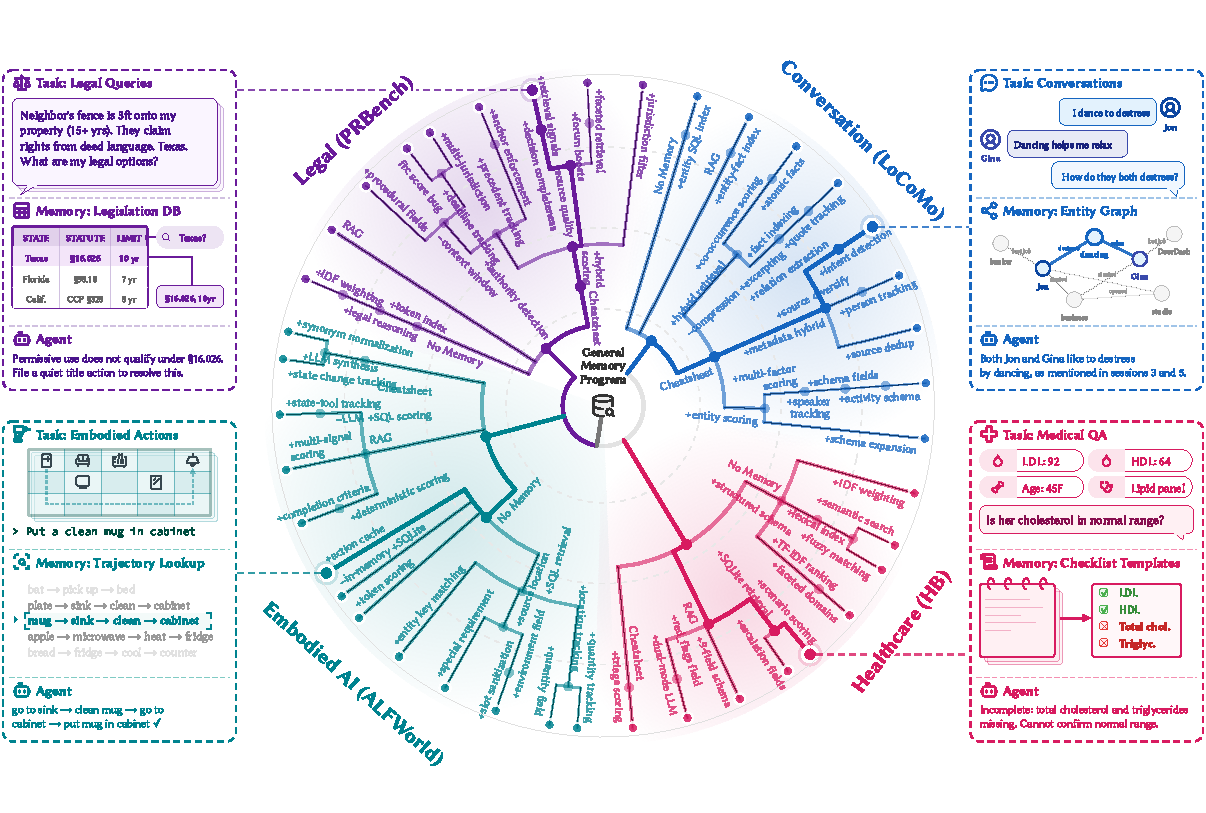
\includegraphics[width=\textwidth]{figures/overview/fig1_combined.pdf}
\captionsetup{type=figure,hypcap=false}
\caption{\textbf{Evolved memory harnesses across tasks.}
The radial tree shows how \sysname{} evolves shared seed programs into task-specialized memory harnesses for LoCoMo, ALFWorld, HealthBench, and PRBench.
The surrounding panels show representative task, memory, and agent behavior for each domain.}
\label{fig:system-overview}
\end{center}
\vspace{-1em}


\begin{abstract}
Large Language Model (LLM) agents rely on a memory harness to write, organize, retrieve, and use past experience.
A harness that works for one task often fails on another, because different tasks like conversations, embodied planning, or expert reasoning require different storage and retrieval behavior.
To address this limitation, we introduce \sysname{}, a method that automatically discovers task-optimized memory programs through reflective code evolution.
Specifically, \sysname{} represents a memory harness as an executable Python program that defines the \textit{Schema}, \textit{Logic}, and \textit{Instruction} components, which are optimized jointly.
We evaluate \sysname{} on four tasks covering conversation, embodied planning, and specialized reasoning.
Our results demonstrate that \sysname{} improves performance over existing static memory harnesses across all evaluated tasks.
Furthermore, the evolved memory programs exhibit structurally distinct processing mechanisms for each evaluated domain.
These findings suggest that every task benefits from its own memory harness, and that memory-program search provides a concrete way to discover it.
\end{abstract}

% === §1 Introduction ===
\section{Introduction}

Agentic systems powered by large language models (LLMs) need a memory harness to reuse past experience across diverse tasks~\citep{zhang2024survey_memory,park2023generative,zhong2024memorybank,wang2024augmenting}.
We use \textit{memory harness} to refer to the components that store, organize, retrieve, and use this experience.
As different task domains require knowledge in different structures, they call for different memory harnesses.
For example, conversational agents need semantic maps of people, events, and preferences to remember user-specific facts (Figure~\ref{fig:system-overview}, top right)~\citep{locomo}, while embodied AI agents need reusable patterns from past trajectories to choose actions in new environments (Figure~\ref{fig:system-overview}, bottom left)~\citep{alfworld}, and specialized reasoning domains may need structured databases (Figure~\ref{fig:system-overview}, top left)~\citep{prbench}.
These requirements encode different assumptions about what to store, how to organize it, and when to retrieve it.
A harness built around one set of assumptions can therefore transfer poorly to another~\citep{structmemeval}.
This raises a practical question: \textit{How can we find the most suitable memory harness for a given task?}

To answer this question, we propose \sysname{}, an evolutionary method that automatically discovers task-optimized memory harnesses for LLM agents.
Specifically, \sysname{} represents a memory harness as a \textit{memory program}: a Python module with a fixed interface consisting of three components, \textit{Schema}, \textit{Logic}, and \textit{Instruction}.
The \textit{Schema} defines the data formats for storage and retrieval, the \textit{Logic} implements the \texttt{read} and \texttt{write} operations, and the \textit{Instruction} guides the agent's interaction with the knowledge base.
These components are jointly optimized through reflective code evolution.
In comparison, although prior works have also searched over and improved agent memory harnesses, their search is typically confined to a narrow, designer-specified space~\citep{zhao2024expel,cai2025flex,memskill,memevolve,gepa}.
\sysname{} searches over the memory harness itself with two mechanisms: a reflector agent that debugs memory program failures and generates targeted improvements, and a population-based program search strategy that balances exploration and exploitation while enforcing constraints on program quality.


We apply \sysname{} to four tasks covering conversation, embodied planning, and specialized reasoning, evaluating its performance against nine competitive baselines across three memory paradigms~\citep{locomo,alfworld,healthbench,prbench}.
Our results indicate that \sysname{} achieves the best overall score and performs robustly on every task; in contrast, the baselines perform well only on specific tasks.
Furthermore, we observe that the optimal memory programs for different tasks are distinct in both structure and procedure.
By exploring a broad memory-program search space, \sysname{} evaluates diverse memory programs to identify the task-optimized memory program.
Together, these results support the view that every task benefits from its own memory harness, discovered as an executable memory program rather than chosen as a fixed design.

In summary, our main contributions are as follows:
\begin{enumerate}
    \item We formulate task-optimized memory harness discovery as \textit{memory-program search}, where an executable Python program jointly specifies Schema, Logic, and Instruction.
    \item We propose \sysname{}, an evolutionary method that optimizes memory harnesses from target-task feedback through reflective code evolution and achieves the strongest overall performance across four tasks compared to competitive generalist memory harnesses.
    \item We perform in-depth analysis over the memory harness space and find that task-optimized memory harnesses are distinct in both structure and procedure across different tasks: conversation, embodied planning, and expert reasoning tasks all require different optimal memory harnesses.
\end{enumerate}

% === §2 Problem Setting ===
% Fig 2: System overview of Mstar
\begin{figure*}[t]
\centering
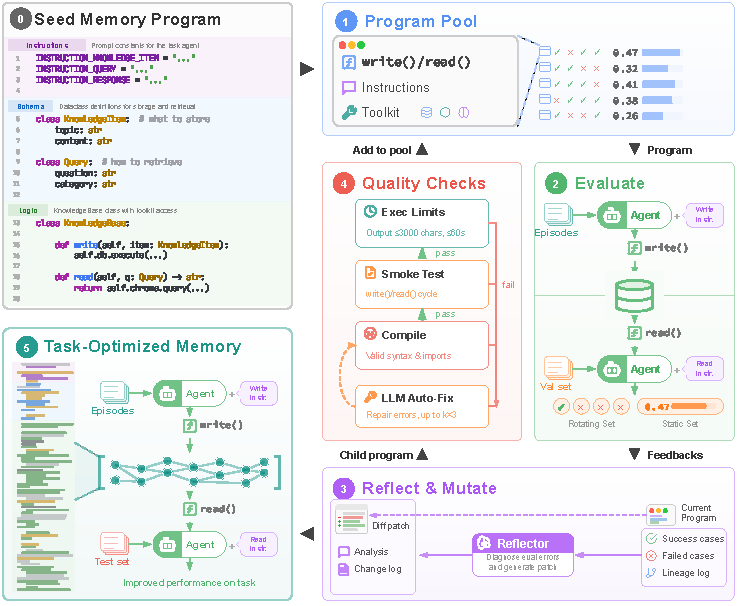
\includegraphics[width=\textwidth]{figures/overview/fig1b_combined.pdf}
\caption{\textbf{System overview of \sysname{}.}
Numbered stages show the workflow from seed memory program~(\textbf{0}) to final test evaluation~(\textbf{5}): population pool~(\textbf{1}), task evaluation~(\textbf{2}), reflective code evolution~(\textbf{3}), and compile/runtime quality checks~(\textbf{4}).}
\label{fig:method-overview}
\vspace{-1em}
\end{figure*}

% §2 Problem Setting

\section{Problem Setting}
\label{sec:problem-setting}

\rev{We consider a task $\mathcal{T} = (\mathcal{D}_\text{e}, \mathcal{D}_\text{v}, \mathcal{D}_\text{t})$, where $\mathcal{D}_\text{e} = \{e_1, \dots, e_N\}$ are trajectories of episodes representing past experiences, $\mathcal{D}_\text{v} = \{(q_1, y_1), \dots, (q_M, y_M)\}$ is a validation set of queries with corresponding ground-truth answers, and $\mathcal{D}_\text{t}$ is a held-out test set used only for final reporting.
An agent $\mathcal{A}$ must memorize information from these past episodes to answer queries from $\mathcal{D}_\text{v}$ and $\mathcal{D}_\text{t}$.}
Specifically, the agent is equipped with a knowledge base $\mathcal{K}$; it observes episodes in $\mathcal{D}_\text{e}$ and extracts knowledge items $k$ to populate this knowledge base $\mathcal{K}$.
At test time, given a query $q_j$, the agent accesses $\mathcal{K}$, which returns relevant context \rev{$c_j = \mathcal{K}.\texttt{read}(q_j)$}.
Building on this retrieved information, the agent then produces its answer or takes an action conditioned on both the query and the context:
\begin{equation}
\hat{y}_j = \mathcal{A}(q_j, \rev{c_j}).
\label{eq:inference}
\end{equation}

\paragraph{Problem Definition: Task-Optimized Memory Program.}
While several prior works have proposed fixed memory methods for agent systems, these generalist structures transfer poorly across task types~\citep{structmemeval}.
To this end, we formalize task-specific memory optimization as search over executable memory programs.
Each program $P$ defines the input and output formats of the knowledge base, its underlying organization method such as a vector database or relational tables, and the agent's policy for when and how to access memory.
Consequently, $P$ describes an open program space that can express many storage and retrieval procedures.
We define $\mathcal{J}(P)$ as the agent's performance on \rev{$\mathcal{D}_\text{v}$} when equipped with a knowledge base instantiated by $P$.
The objective is to find the optimal memory program $P^*$ that maximizes this performance metric:
\begin{equation}
P^* = \arg\max_P \mathcal{J}(P).
\label{eq:objective}
\end{equation}
In the next section, we address how we can automatically discover the optimal memory program for a given task. Specifically, we propose a framework that uses reflective code evolution to search this program space.


% === §3 Method ===
% §3 Mstar
% Reference: Knowledge/Wiki/Method Section Framework.md

\section{Method}
\label{sec:mstar}

% Fig: System overview moved to Introduction for earlier visibility

Figure~\ref{fig:method-overview} gives an overview of the system \sysname{}, a reflective code evolution method that automatically discovers task-optimized memory programs.
Specifically, \sysname{} consists of three main components: (1) representing the memory-program search space in code (Section~\ref{sec:search-space}), (2) reflective code evolution (Section~\ref{sec:reflection}), and (3) population-based program search (Section~\ref{sec:population}).

\subsection{Representing the Memory-Program Search Space in Code}
\label{sec:search-space}

We represent each memory program as an executable Python module with a fixed interface.
% In contrast, recent works on evolutionary memory typically restrict optimization to predefined memory methods~\citep{cai2025flex, memevolve} or to textual optimization at the prompt level~\citep{memskill, gepa}.
To define a broad memory-program search space, each memory program simultaneously controls three key components of the knowledge base: \textit{Schema}, \textit{Logic}, and \textit{Instruction}.
In addition, the program has access to a standardized \textit{Toolkit}.

\begin{itemize}
    \item \textbf{Schema.}\looseness=-1
    The Schema specifies the data formats that the knowledge base accepts for writing and querying.
    For example, the input format can range from structured data with timestamps to natural language insights.
    We implement the Schema using Python dataclasses.
    As a result, when the agent needs to write or query information, it instantiates these dataclass types and passes them into the memory program for parsing.

    \item \textbf{Logic.}
    The Logic defines the backend operations of the knowledge base when processing and storing Schema-formatted inputs and queries.
    This component can include operations such as computing embeddings, managing SQL tables, or calling an LLM for secondary data processing.
    Specifically, the Logic exposes \texttt{write} and \texttt{read} functions, which are executed whenever the agent performs write or read actions.

    \item \textbf{Instruction.}
    The Instruction defines how the agent interacts with the knowledge base.
    This includes how to extract information from observed episodes, how to formulate queries, and how to interpret the results returned by the knowledge base.
    We define the Instruction through constant prompt strings.
    These instruction constants are inserted into the system prompt when the agent executes corresponding write, query, and response actions.

    \item \textbf{Toolkit.}
    Within the memory-program search space, we allow the memory program to use various data structures and external tools.
    We provide a set of whitelisted components, including lists, heaps, relational databases, vector databases, and LLM endpoints.
    The Toolkit enables memory programs to implement complex storage and retrieval procedures.
\end{itemize}

\subsection{Reflective Code Evolution}
\label{sec:reflection}

Representing a memory program using executable code places memory-program search in an enormous search space.
Inspired by recent evolutionary algorithm discovery methods, we design a reflective code evolution process that iteratively refines memory programs using validation feedback~\citep{romera2024funsearch,chen2023evoprompting,deepmind2025alphaevolve}.
Specifically, this process consists of three stages: sampling feedback from a validation loop, iterative refinement via a coding agent, and constraint checking with automated repair before the candidate is scored.

\textbf{Sampling feedback from the validation loop.}
We use a set of episodes and validation queries to evaluate a memory program.
The validation queries are partitioned into a \textit{static} set, which remains constant across all iterations, and a \textit{rotating} set, which changes in each iteration similar to mini-batches in training.
During validation, the agent initiates a query to the knowledge base for each sample in both the rotating and static sets and \rev{uses} the returned information to generate a response or take an action.
The aggregated score on the static validation set serves as the performance metric for the current memory program.
Meanwhile, the generated trajectories on \rev{the} rotating set are used as feedback to improve the program later.
% We partition the validation data into static and dynamic sets because the rotating validation set provides targeted feedback without leaking information from the static set, preventing evaluation contamination.
% Simultaneously, using an identical static validation set ensures that the scores remain comparable across different memory programs.

\textbf{Coding agent iteration.}
We employ a coding agent to iteratively update the current memory program to improve performance and fix potential bugs.
We provide the coding agent the execution trajectories from the read and write processes, underperforming samples from the rotating validation set, and the change logs from prior iterations along with their corresponding scores.
Based on this information, the coding agent analyzes whether the read and write operations function as expected, identifies the root causes of underperforming cases, and determines which past improvements were effective.
Consequently, the coding agent generates a code patch to apply to the current program and produces a new change log to guide future iterations.
The complete prompt template is provided in Appendix~\ref{app:prompts}.

\textbf{Constraint checks and automated repair.}
Before applying the updated memory program, the code evolution process executes a set of runtime checks to ensure its quality.
If any check fails, the memory program and its corresponding error messages are resubmitted to the coding agent for repair.
\rev{These checks prevent low-quality programs from consuming excessive computational resources, and any program that still fails after a fixed number of repair attempts is discarded.}

\subsection{Population-Based Program Search}
\label{sec:population}

Unlike function search or prompt optimization, evaluating a memory program in \sysname{} can be highly expensive.
For any program change, the agent must regenerate episode knowledge and evaluate the program on validation tasks.
Therefore, the search procedure should reuse useful intermediate programs rather than follow a single update trajectory.

Instead of continuously updating a single program, which can cause the evolution algorithm to fall into local optima, we maintain a program pool.
We initialize the search with a small set of simple seed programs (Appendix~\ref{app:seeds}).
In each iteration, we sample a parent program from the pool with probability biased toward higher validation scores.
Specifically, the probability \rev{$\Pr(P_i)$ of selecting program $P_i$} from the pool is computed as:
\begin{equation}
    \rev{\Pr(P_i) = \frac{\exp(\mathcal{J}(P_i) / \tau)}{\sum_{j} \exp(\mathcal{J}(P_j) / \tau)}},
\end{equation}
where \rev{$\mathcal{J}(\cdot)$ is the static validation score (Eq.~\ref{eq:objective})} and $\tau$ is the softmax temperature.
The coding agent then applies a reflective mutation step to the selected parent, and the resulting child program is added back to the pool.
This design balances exploration and exploitation; top-performing programs have a greater chance of being selected for improvement, yet lower-scoring programs retain a non-zero probability of being explored.
We use additional subset-selection procedures to reduce evaluation cost, and describe these implementation details in Appendix~\ref{app:representative-subset}.

Overall, \sysname{} provides an efficient reflective code evolution procedure for memory-program search.
In the following section, we provide an empirical analysis to validate our method.

% Table 1: Main Results
% PURPOSE: Primary evidence — Ours vs baselines across benchmarks.
%   Three baseline categories with colored group headers.
%   LoCoMo: token F1 / LLM judge. ALFWorld: success rate. HB/PR: rubric score.
\begin{table*}[t]
    \centering
    \footnotesize
    \setlength{\tabcolsep}{3.5pt}
    \caption{\textbf{Main results across four benchmark families.}
    Columns report LoCoMo token F1 and LLM-judge score, ALFWorld success rate, HealthBench rubric score, and PRBench rubric score.
    Baselines are grouped by memory paradigm.
    Best per column in \textbf{bold}, second best in \second{green}.}
    \vspace{-0.5em}
    \label{tab:main-results}
    % Use tabularx for full text width; X column absorbs slack on the method name.
    \newcolumntype{Y}{>{\centering\arraybackslash}X}
    \begin{tabularx}{\textwidth}{l *{2}{Y} *{2}{Y} *{2}{Y} *{2}{Y}}
        \toprule
        \rowcolor{gray!10}
         & \multicolumn{2}{c}{\textbf{LoCoMo}} & \multicolumn{2}{c}{\textbf{ALFWorld}} & \multicolumn{2}{c}{\textbf{HealthBench}} & \multicolumn{2}{c}{\textbf{PRBench}} \\
        \cmidrule(lr){2-3} \cmidrule(lr){4-5} \cmidrule(lr){6-7} \cmidrule(lr){8-9}
        \rowcolor{gray!10}
        \textbf{Method} & \textbf{F1} & \textbf{L-J} & \textbf{Unseen} & \textbf{Seen} & \textbf{Data} & \textbf{Emerg.} & \textbf{Legal} & \textbf{Finance} \\
        \midrule
        % --- No Memory (standalone, above first group) ---
        No Memory            & 0.036 & 0.030 & 0.738 & 0.640 & 0.242 & 0.429 & 0.431 & 0.269 \\
        \midrule
        % --- Group 1: Retrieval-based Systems (Memorizing Episodes) ---
        \multicolumn{9}{l}{\textit{\textbf{Retrieval-based Systems} (Memorizing Episodes)}} \\
        \midrule
        \quad Vector Search   & 0.256 & 0.400 & 0.643 & 0.720 & 0.264 & 0.400 & 0.466 & 0.308 \\
        \quad G-Memory        & 0.224 & 0.380 & 0.690 & 0.560 & 0.309 & 0.447 & 0.499 & 0.318 \\
        \quad Mem0            & \second{0.373} & \second{0.540} & 0.738 & 0.640 & 0.216 & 0.413 & 0.450 & 0.321 \\
        \midrule
        % --- Group 2: Self-evolution Systems (Memorizing Experiences) ---
        \multicolumn{9}{l}{\textit{\textbf{Self-evolution Systems} (Memorizing Experiences)}} \\
        \midrule
        \quad Trajectory Retrieval & 0.276 & 0.420 & 0.714 & \second{0.780} & 0.265 & 0.442 & 0.480 & 0.304 \\
        \quad ReasoningBank        & 0.194 & 0.380 & 0.738 & 0.580 & 0.315 & 0.470 & 0.508 & 0.330 \\
        \quad Dynamic Cheatsheet   & 0.124 & 0.190 & 0.619 & 0.480 & 0.286 & \second{0.487} & 0.474 & 0.327 \\
        \midrule
        % --- Group 3: Prompt-optimizing systems (learned prompts) ---
        \multicolumn{9}{l}{\textit{\textbf{Prompt-optimizing Systems} (Learned Prompts)}} \\
        \midrule
        \quad GEPA                 & 0.132 & 0.190 & \second{0.857} & 0.720 & 0.304 & 0.466 & \second{0.568} & \second{0.449} \\
        \quad GEPA + Vector Search & 0.300 & 0.390 & 0.810 & \textbf{0.820} & \second{0.327} & 0.484 & 0.554 & 0.411 \\
        \midrule
        % --- Ours ---
        \rowcolor{green!10}
        \textbf{\sysname{}} & \textbf{0.459} & \textbf{0.610} & \textbf{0.881} & 0.700 & \textbf{0.390} & \textbf{0.493} & \textbf{0.660} & \textbf{0.586} \\
        \bottomrule
    \end{tabularx}%
    \vspace{-1em}
\end{table*}



% === §4 Experimental Setup ===
% === §3 Experimental Setup ===
\section{Experimental Setup}
\label{sec:experimental-setup}

\looseness=-1
We evaluate \sysname{} on four benchmark families with seven domain configurations, covering long-term conversational question answering, embodied household task completion, medical decision support, and professional legal and financial reasoning.
For each configuration, we run 20 evolution iterations, select the best memory program on validation, and report performance on a held-out test split.
We use GPT-5.4 Mini as the task agent and GPT-5.3-Codex as the coding agent in reflective code evolution~\citep{openai2026gpt54mini,openai2026gpt53codex}.
Additional dataset splits, hyperparameters, evaluation protocols, computational costs, and pseudocode are provided in Appendix~\ref{app:datasets}, Appendix~\ref{app:hyperparameters}, Appendix~\ref{app:eval-protocols}, Appendix~\ref{app:cost}, and Appendix~\ref{app:algorithm}.

\noindent\textbf{Benchmarks.}
We use \rev{LoCoMo~\citep{locomo}} to test long-term conversational memory, \rev{ALFWorld~\citep{alfworld}} to test memory use in embodied planning, \rev{HealthBench~\citep{healthbench}} to test rubric-graded health reasoning, and \rev{PRBench~\citep{prbench}} to test professional legal and financial reasoning.
Together, these benchmarks cover retrieval-heavy question answering, interactive decision making, and specialized reasoning under structured evaluation.
Dataset construction details are provided in Appendix~\ref{app:datasets}, and metric details are provided in Appendix~\ref{app:eval-protocols} for all seven benchmark configurations.

\noindent\textbf{Baselines.}
We compare \sysname{} with nine baselines, including a no-memory control and eight memory-based methods spanning three paradigms, as summarized in Table~\ref{tab:main-results}.
These baselines cover direct answering without external memory, retrieval-based memory over stored observations, self-evolving memories that distill reusable experience, and prompt-optimization methods with and without vector retrieval~\citep{rag,alma,ouyang2025reasoningbank,gepa}.
Detailed baseline implementations are provided in Appendix~\ref{app:baselines}, with implementation notes for every baseline.


% === §5 Results ===
% === Table 1: Main Results ===

% === Fig 3: Evolution Trajectory (D3 version) ===
% Fig 3: Evolution Trajectory (D3 version)
\begin{figure*}[t]
\centering
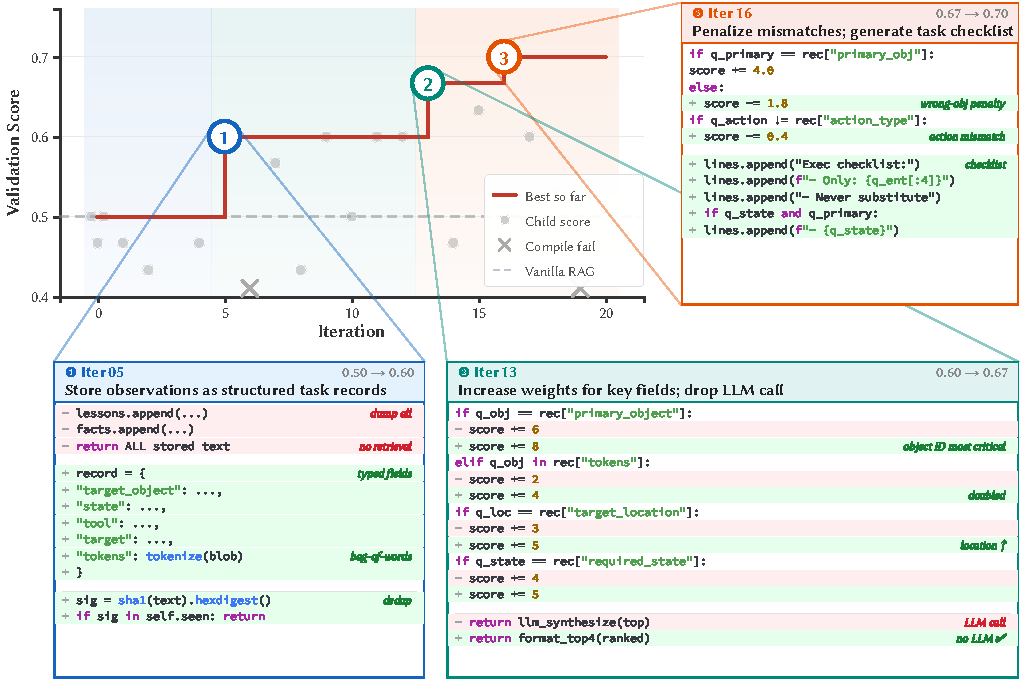
\includegraphics[width=\textwidth]{figures/trajectory/fig3_d3.pdf}
\caption{\textbf{ALFWorld evolution trajectory.}
The main panel plots each child program's validation score and the best score so far across 20 evolution iterations, with crosses marking compile failures and the dashed line marking the Vanilla RAG baseline.
Numbered panels highlight representative code changes that structure task records, reweight retrieval, and add mismatch penalties and execution checklists for selecting the next action.}
\label{fig:evolution-trajectory}
\vspace{-1em}
\end{figure*}



\section{Results}
\label{sec:results}

We organize the analysis around three questions: whether memory-program search improves task performance, whether the resulting programs differ structurally across tasks, and which evolved components drive the gains.

\paragraph{Reflective code evolution progressively discovers better memory programs.}\looseness=-1
Table~\ref{tab:main-results} shows that \sysname{} achieves the highest score on seven of eight reported metrics.
Compared with the best baseline in each winning metric, the relative improvement is up to 31\%, with the largest gains on LoCoMo and PRBench.
The strongest baseline varies by task, indicating that existing memory methods have task-dependent strengths.
GEPA is competitive on ALFWorld and PRBench, while Mem0, GEPA+Vector Search, and Dynamic Cheatsheet lead the baselines on LoCoMo and HealthBench.
In comparison, \sysname{} achieves the best overall performance.
This pattern suggests that executable code search reaches useful memory designs beyond the strongest fixed baselines.
Figure~\ref{fig:evolution-trajectory} shows the ALFWorld evolution trajectory.
The evolved memory program improves steadily over iterations, with the reflector producing task-specific changes at different stages of search.
Early edits build a usable task-record schema that captures objects, locations, and state changes from demonstrations.
Later edits refine retrieval weights and add action-selection checks, allowing the agent to retrieve more relevant trajectory patterns and choose actions more reliably.

\paragraph{Different tasks produce structurally distinct optimal memory programs.}
% Table 2: Ablation study on LoCoMo
\begin{wraptable}{r}{0.44\textwidth}
    % \vspace{-1.2em}
    \centering
    \footnotesize
    \caption{\textbf{Ablation study on LoCoMo.}
    Rows report the full system and variants that remove or alter one design choice; metric is token F1.
    $\Delta$ reports absolute change from the full system.}
    % \vspace{-0.5em}
    \label{tab:ablation}
    \begin{tabular}{@{}lcc@{}}
        \toprule
        \rowcolor{gray!10}
        \textbf{Variant} & \textbf{F1} & \textbf{$\Delta$} \\
        \midrule
        \rowcolor{green!10}
        \sysname{}                           & 0.459  & ---      \\
        \quad $-$ Instruction                 & 0.353  & $-$0.106 \\
        \quad $-$ Code                        & 0.256  & $-$0.203 \\
        \quad Max parent selection          & 0.381  & $-$0.078 \\
        \quad $-$ Diversity                   & 0.318  & $-$0.141 \\
        \bottomrule
    \end{tabular}%
    \vspace{-1em}
\end{wraptable}


% fig5.tex — Program embedding landscape (Observation 4)
% Generated from fig5.html via Puppeteer → fig5.pdf

\begin{figure*}[t]
\centering
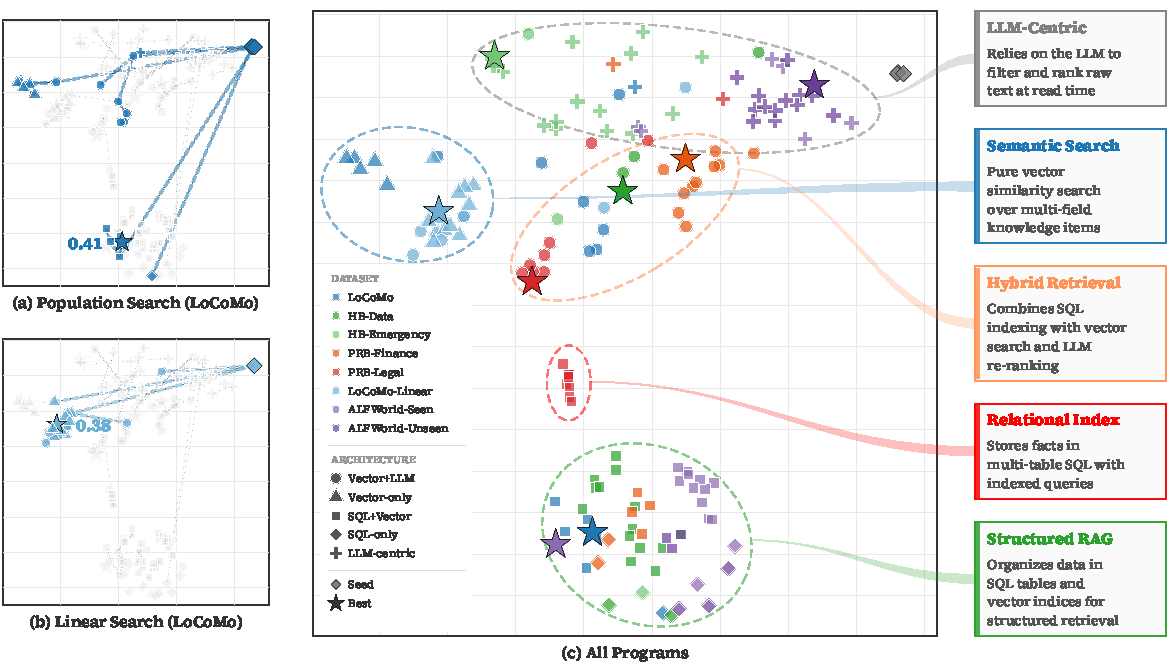
\includegraphics[width=\textwidth]{figures/landscape/fig5.pdf}
\caption{%
  \textbf{Program embedding landscape.}
  Each evolved program is embedded with a code embedding model and projected to 2D via t-SNE~\citep{vandermaaten2008tsne}.
  \textbf{(a,\,b)}~Population-based search (\sysname{}) and linear search, with colored edges tracing parent-child lineage.
  \textbf{(c)}~All programs from the evaluated configurations and the LoCoMo linear-search ablation, colored by configuration.
  Marker shapes denote the storage architecture discovered by evolution: circles for vector\,+\,LLM, triangles for vector-only, squares for SQL\,+\,vector, rotated squares for SQL-only, and crosses for LLM-centric designs; diamonds mark seed programs and stars mark the best program for each configuration.
}
\label{fig:landscape}
\end{figure*}


To understand how \sysname{} adapts memory program structure to different tasks, we visualize the program embedding landscape accumulated during evolution (Figure~\ref{fig:landscape}).
For each task and iteration, we first sanitize the program by replacing strings and variable names with placeholders so that the embedding emphasizes structural differences.
We then embed the sanitized programs with a code embedding model and project them with t-SNE~\citep{vandermaaten2008tsne}.
The projection places the best programs for different benchmark configurations in separate regions, with markers indicating different storage architectures.
For example, the best ALFWorld program uses a compact SQLite action cache with read-time LLM synthesis.
The best LoCoMo program uses ChromaDB semantic retrieval together with SQLite lexical and metadata scoring.
Appendix~\ref{app:evolved-comparison} reports structural summaries, and the supplementary material includes full code for all best programs.

% Fig 4: Cross-task transfer of evolved memory programs
\begin{figure*}[t]
\centering
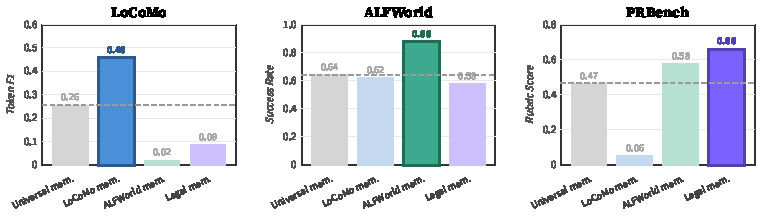
\includegraphics[width=\textwidth]{figures/comparison/fig4.pdf}
\caption{\textbf{Cross-task transfer of evolved memory programs.}
Each panel fixes one target benchmark and compares memory programs evolved on different source benchmarks.
Highlighted bars mark native-task programs, and the dashed line marks the universal seed baseline.}
\label{fig:task-optimized-memory}
\vspace{-1em}
\end{figure*}


To further test whether these structures are task-specific, we evaluate the best evolved program from each source task on other target tasks (Figure~\ref{fig:task-optimized-memory}).
In all three targets, the native evolved program outperforms transferred programs from other benchmarks.
Five of six transferred programs perform worse than the universal seed baseline.
This pattern suggests that memory program structure should be optimized together with the target task.


\paragraph{Joint evolution of structure and policy enables task-specific adaptation.}
Table~\ref{tab:ablation} isolates key design choices on LoCoMo.
Each variant removes one component of \sysname{}: \textit{$-$\,Instruction} lets only the code evolve and keeps the prompt instructions fixed; \textit{$-$\,Code} does the opposite, evolving only the prompt instructions while keeping the code at the Vector Search seed; \textit{Max parent selection} always picks the highest-scoring parent instead of sampling by softmax; and \textit{$-$\,Diversity} drops the population pool and mutates only the current best program at each iteration.
\textit{$-$\,Code} gives the largest drop, reducing F1 by 0.203.
\textit{$-$\,Instruction} reduces F1 by 0.106.
The full system also scores above \textit{Max parent selection} and \textit{$-$\,Diversity}.
These results indicate that joint optimization of program Logic and Instruction gives the strongest LoCoMo result.

% === Table 2: Ablation ===


% === §6 Discussion ===
\section{Discussion}
\label{sec:discussion}

In this section, we examine three properties of reflective code evolution: search diversity, seed stability, and category effects.

\paragraph{How does evolution explore the program space?}

Figure~\ref{fig:landscape}(c) provides another view of the search process.
Evolved programs form several regions with different storage designs, including LLM-centric, vector-only, SQL-only, SQL+vector, and vector+LLM programs.
Programs from different benchmarks often appear in the same regions.
This pattern suggests that evolution can try common storage designs before adapting them to a task.
Figure~\ref{fig:landscape}(a,b) further compares population-based search with a linear variant.
The linear variant starts from one empty seed and repeatedly mutates only the current best program\rev{; this corresponds to the $-$\,Diversity ablation in Table~\ref{tab:ablation}}.
Population search keeps multiple candidates active, so later mutations can draw from more than one candidate lineage.
The LoCoMo ablation matches this interpretation: removing diversity reduces test F1 from 0.459 to 0.318, and max sampling with multiple starters reaches 0.381 (Table~\ref{tab:ablation}).
These results suggest that population search helps preserve promising program lineages under a small iteration budget.

\paragraph{Is evolution stable across random seeds?}

% === Table: Stability Across Seeds ===
% Table: Stability Across Seeds
\begin{wraptable}{r}{0.64\textwidth}
    \vspace{-1.2em}
    \centering
    \scriptsize
    \caption{\textbf{Stability across evolution seeds.}
    Mean and std.\ are computed over five independent stability runs with random seeds; metrics match the primary columns in \autoref{tab:main-results}.
    CV is the coefficient of variation in percent, Best Baseline is the strongest fixed baseline, and Win is the number of seeds above that baseline.}
    \vspace{-0.5em}
    \label{tab:stability}
    \begin{tabularx}{\linewidth}{@{}l >{\centering\arraybackslash}X >{\centering\arraybackslash}p{0.6cm} >{\centering\arraybackslash}p{2.6cm} >{\centering\arraybackslash}p{0.6cm}@{}}
        \toprule
        \rowcolor{gray!10}
        \textbf{Benchmark} & \textbf{Mean{\scriptsize$\pm$Std}} & \textbf{CV} & \textbf{Best Baseline} & \textbf{Win} \\
        \midrule
        LoCoMo          & $\rev{0.421_{\pm0.042}}$ & \rev{10.0} & 0.373 {\scriptsize(Mem0)}         & 4/5 \\
        HB Data         & $0.391_{\pm0.023}$ &  5.9 & 0.327 {\scriptsize(GEPA{+}VS)}    & 5/5 \\
        PR Finance      & $0.561_{\pm0.032}$ &  5.7 & 0.449 {\scriptsize(GEPA)}          & 5/5 \\
        \bottomrule
    \end{tabularx}%
    \vspace{-1em}
\end{wraptable}


A practical concern for evolutionary methods is sensitivity to random seeds, especially under a 20-iteration budget in which discovery quality can depend on early mutations.
To evaluate this effect, Table~\ref{tab:stability} reports test scores from five independent runs on three benchmarks.
Across all benchmarks, the coefficient of variation remains \rev{at or below 10\%}, which indicates stable outcomes with moderate variance.
Across the 15 runs, 14 outperform the strongest baseline, supporting consistent gains across initializations.
Appendix~\ref{app:stability} provides full per-seed scores and validation trajectories.

\paragraph{Does evolution improve performance uniformly?}

% === Table: Per-Category Breakdown (combined) ===
% Table: Per-Category Breakdown (combined)
\begin{table*}[t]
    \centering
    \small
    \caption{\textbf{Per-category performance breakdown.}
    \textbf{(a)}~ALFWorld Unseen success rate by task type.
    \textbf{(b)}~LoCoMo token F1 by query type.
    $n$ is the number of test episodes or test queries per category.
    Min reports the minimum score across shown categories.
    Best per column in \textbf{bold}.}
    \vspace{-0.5em}
    \label{tab:per-category}
    \resizebox{\textwidth}{!}{%
    \begin{tabular}{@{}l ccccc c !{\vrule width 0.6pt} cccc c@{}}
        \toprule
        \rowcolor{gray!10}
        & \multicolumn{6}{c!{\vrule width 0.6pt}}{\textbf{(a) ALFWorld Unseen}} & \multicolumn{5}{c}{\textbf{(b) LoCoMo}} \\
        \cmidrule(r){2-7} \cmidrule(l){8-12}
        \rowcolor{gray!10}
        & \textbf{Simple} & \textbf{Clean} & \textbf{Cool} & \textbf{Heat} & \textbf{2-Obj} &
        & \textbf{Single} & \textbf{Temp.} & \textbf{Causal} & \textbf{Open} & \\
        \rowcolor{gray!10}
        & \footnotesize$(n{=}8)$ & \footnotesize$(n{=}11)$ & \footnotesize$(n{=}7)$ & \footnotesize$(n{=}6)$ & \footnotesize$(n{=}8)$ & \textbf{Min}
        & \footnotesize$(n{=}18)$ & \footnotesize$(n{=}18)$ & \footnotesize$(n{=}9)$ & \footnotesize$(n{=}55)$ & \textbf{Min} \\
        \midrule
        No Memory            & 0.88 & 0.82 & 0.57 & 0.83 & 0.62 & 0.57 & 0.02 & 0.00 & 0.11 & 0.04 & 0.00 \\
        Mem0                 & 0.88 & 0.64 & 0.57 & \textbf{1.00} & 0.75 & 0.57 & \textbf{0.33} & 0.26 & 0.37 & 0.43 & 0.26 \\
        Trajectory Retrieval & 0.75 & 0.73 & 0.71 & 0.67 & 0.75 & 0.67 & 0.18 & 0.33 & 0.34 & 0.28 & 0.18 \\
        GEPA + Vector Search & 0.88 & \textbf{1.00} & 0.57 & \textbf{1.00} & 0.62 & 0.57 & 0.15 & \textbf{0.38} & \textbf{0.39} & 0.31 & 0.15 \\
        \rowcolor{green!10}
        \sysname{}      & 0.88 & 0.91 & \textbf{1.00} & 0.83 & 0.75 & \textbf{0.75} & \textbf{0.33} & 0.19 & 0.35 & \textbf{0.51} & 0.19 \\
        \bottomrule
    \end{tabular}}%
    \vspace{-1em}
\end{table*}


Table~\ref{tab:per-category} disaggregates the results in Table~\ref{tab:main-results} by category (full per-category tables are in Appendix~\ref{app:per-category}).
On ALFWorld Unseen, \sysname{} raises the worst category score to 0.75, above the best baseline floor among the methods shown (0.67).
This pattern suggests that the evolved action cache addresses failure modes that fixed designs leave exposed across task types.
On LoCoMo, the gains are less uniform: \sysname{} is strongest on open-domain questions and tied on single-hop recall, while Mem0 and GEPA+Vector Search remain stronger on temporal and causal questions.
This split suggests that an aggregate objective can improve the overall score while leaving lower-frequency or harder categories underserved.


% === §7 Related Work ===
% §6 Related Work
% Structure: MemSkill §2 sentence-level skeleton
% Prose quality: GEPA-level (causal chains, specific mechanisms, dense)
% Target: ~314 words ± 15%

\section{Related Work}

\noindent\textbf{Memory for LLM Agents.}
Prior work on agent memory builds external stores from interaction histories~\citep{zhang2024survey_memory}: typical pipelines extract salient information, retrieve relevant entries for a new query, and update via consolidation or pruning~\citep{park2023generative,zhong2024memorybank,wang2024augmenting}.
Recent systems learn richer policies; MemSkill~\citep{memskill} selects natural-language skills via an RL controller, and AWM~\citep{wang2024awm} induces reusable workflows from successful trajectories.
Concurrent work on self-evolving memory stays within closed design spaces, e.g., MemEvolve~\citep{memevolve} searches over four predefined modules (encode, store, retrieve, manage).
All commit to a fixed representation at design time and cannot express task-specific computational logic such as relational schemas or stateful aggregations.
By contrast, we search over executable Python programs that implement arbitrary data structures and retrieval logic, subsuming these closed spaces.

\noindent\textbf{Self-Evolving Agents.}~\looseness=-1
Self-evolving LLM agents improve from interaction experience without gradient-based updates~\citep{gao2025survey_selfevolving}.
ExpeL~\citep{zhao2024expel} distills trajectories into editable natural-language insights, FLEX~\citep{cai2025flex} builds an experience library via continual reflection, and a complementary line automates agent design through meta-optimization (ADAS~\citep{hu2024adas}), skill synthesis (Voyager~\citep{wang2023voyager}), and verbal self-critique (Reflexion~\citep{shinn2023reflexion}).
These systems evolve text-level artifacts that the LLM must re-interpret at runtime; \sysname{} instead evolves deterministic code, reducing interpretation variance and enabling explicit data structures and retrieval logic in each memory program.

\noindent\textbf{Program Search with Language Models. }
Using LLMs as mutation operators has yielded solutions surpassing human heuristics in combinatorial optimization~\citep{romera2024funsearch}, neural architecture search~\citep{chen2023evoprompting}, and algorithmic discovery~\citep{deepmind2025alphaevolve}.
Closest to our work, GEPA~\citep{gepa} mutates every prompt in a compound AI system via reflective natural-language updates with Pareto-front candidate selection.
\sysname{} applies the same paradigm to executable memory programs; because generated code can fail to compile or violate runtime constraints, we add a compile-fix loop and runtime violation recovery that are unnecessary in prompt evolution (Section~\ref{sec:reflection}).


% === §8 Conclusion ===
\section{Conclusion}

We introduced \sysname{}, a method that discovers task-optimized memory programs for large language model agents through reflective code evolution.
By representing a memory harness as executable Python code with Schema, Logic, and Instruction, \sysname{} turns memory design into a memory-program search problem.
Across four benchmarks, the evolved programs outperform strong memory baselines and develop distinct storage, retrieval, and action workflows for different domains.
These results support the view that agent memory should be optimized for the target task, and that memory-program search provides a practical path toward this goal.
Future work will study more sample-efficient search strategies and extend this framework to broader classes of agent tasks.

\bibliographystyle{plainnat}
\bibliography{references}

% === Appendix ===

\appendix

\section*{Appendix}

\vspace{0.4em}

\newcommand{\appsection}[3]{%
  \noindent\colorbox{gray!7}{\parbox{\dimexpr\linewidth-2\fboxsep}{%
    \textbf{\textcolor{cyan!70!black}{#1}\hspace{0.5em}#2}\hfill\pageref{#3}%
  }}\par\vspace{0.05em}%
}
\newcommand{\appsubsection}[2]{%
  \noindent\hspace{1em}#1\dotfill\pageref{#2}\par%
}

\begingroup
\scriptsize
\begin{center}
\textbf{\large Table of Contents}
\end{center}

\vspace{0.25em}
\hrule
\vspace{0.35em}

\appsection{A}{Reflective Code Evolution Algorithm}{app:algorithm}
\appsubsection{A.1\hspace{0.5em}Evolution Loop}{alg:evolution-loop}
\appsubsection{A.2\hspace{0.5em}Split Evaluation}{alg:split-eval}

\vspace{0.1em}
\appsection{B}{Benchmarks and Dataset Details}{app:datasets}
\appsubsection{B.1\hspace{0.5em}Dataset Splits}{app:dataset-splits}
\appsubsection{B.2\hspace{0.5em}LoCoMo}{app:dataset-locomo}
\appsubsection{B.3\hspace{0.5em}ALFWorld}{app:dataset-alfworld}
\appsubsection{B.4\hspace{0.5em}HealthBench}{app:dataset-healthbench}
\appsubsection{B.5\hspace{0.5em}PRBench}{app:dataset-prbench}

\vspace{0.1em}
\appsection{C}{Baseline Methods}{app:baselines}
\appsubsection{C.1\hspace{0.5em}No Memory}{app:baseline-no-memory}
\appsubsection{C.2\hspace{0.5em}Retrieval-Based Systems}{app:baseline-retrieval}
\appsubsection{C.3\hspace{0.5em}Self-Evolution Systems}{app:baseline-self-evolution}
\appsubsection{C.4\hspace{0.5em}Prompt-Optimizing Systems}{app:baseline-prompt}

\vspace{0.1em}
\appsection{D}{Experiment Configuration}{app:experiment-config}
\appsubsection{D.1\hspace{0.5em}Computational Cost}{app:cost}
\appsubsection{D.2\hspace{0.5em}Hyperparameters}{app:hyperparameters}
\appsubsection{D.3\hspace{0.5em}Representative Subset Selection}{app:representative-subset}

\vspace{0.1em}
\appsection{E}{Seed Programs}{app:seeds}
\appsubsection{E.1\hspace{0.5em}Vector Search}{app:seed-vector-search}
\appsubsection{E.2\hspace{0.5em}LLM Summarizer}{app:seed-llm-summarizer}
\appsubsection{E.3\hspace{0.5em}Experience Learner}{app:seed-experience-learner}

\vspace{0.1em}
\appsection{F}{Evolved Programs}{app:evolved-programs}
\appsubsection{F.1\hspace{0.5em}ALFWorld: Deterministic Action Cache}{app:evolved-alfworld}
\appsubsection{F.2\hspace{0.5em}LoCoMo: Multi-Signal Episodic Index}{app:evolved-locomo}
\appsubsection{F.3\hspace{0.5em}HealthBench and PRBench Program Sketches}{app:evolved-health-pr}
\appsubsection{F.4\hspace{0.5em}Cross-Benchmark Structural Comparison}{app:evolved-comparison}

\vspace{0.1em}
\appsection{G}{Prompt Templates and Mutation Interface}{app:prompts}
\appsubsection{G.1\hspace{0.5em}Task Agent Prompts}{app:task-agent-prompts}
\appsubsection{G.2\hspace{0.5em}Reflector Prompt}{app:reflector-prompt}
\appsubsection{G.3\hspace{0.5em}Compile-Fix Prompt}{app:compile-fix-prompt}

\vspace{0.1em}
\appsection{H}{Evaluation Protocols}{app:eval-protocols}
\appsubsection{H.1\hspace{0.5em}Token F1 (LoCoMo)}{app:metric-token-f1}
\appsubsection{H.2\hspace{0.5em}Binary Success (ALFWorld)}{app:metric-binary-success}
\appsubsection{H.3\hspace{0.5em}Rubric-Based Scoring}{app:metric-rubric}

\vspace{0.1em}
\appsection{I}{Extended Results}{app:extended-results}
\appsubsection{I.1\hspace{0.5em}Complete Per-Category Results}{app:per-category}
\appsubsection{I.2\hspace{0.5em}Multi-Seed Stability Results}{app:stability}

\vspace{0.1em}
\appsection{J}{Limitations}{app:limitations}

\vspace{0.1em}
\appsection{K}{Broader Impact}{app:broader-impact}

\vspace{0.1em}
\appsection{L}{LLM Usage}{app:llm-usage}

\vspace{0.3em}
\hrule
\endgroup

\section{Reflective Code Evolution Algorithm}
\label{app:algorithm}

\begin{algorithm}[!htbp]
\caption{\textbf{Reflective code evolution for memory-program search.}
The left panel gives the population-based evolution loop, and the right panel gives split evaluation for a candidate program.}
\label{alg:evolution}
\begin{minipage}[t]{0.47\linewidth}
\textbf{(a) Evolution Loop} \label{alg:evolution-loop}
\begin{algorithmic}[1]
\REQUIRE Seed programs $\{S_1,\ldots,S_K\}$, budget $B$, temp.\ $\tau$
\REQUIRE Episodes $D_\text{e}$, static val $D_\text{v}$, rotate pool $D_\text{r}$
\ENSURE Best program $P^*$
\STATE $\mathcal{P} \gets \emptyset$
\FOR{$i = 1$ \TO $K$}
    \STATE $(J_i, \_) \gets \textsc{Eval}(S_i, D_\text{e}, D_\text{v})$
    \STATE $\mathcal{P} \gets \mathcal{P} \cup \{(S_i, J_i)\}$
\ENDFOR
\FOR{$t = 1$ \TO $B$}
    \STATE $P_\text{par} \gets \textsc{SoftmaxSample}(\mathcal{P}, \tau)$
    \STATE $\tilde{D} \gets \textsc{Sample}(D_\text{r},\, n_r)$
    \STATE $(\_, \mathcal{R}) \gets \textsc{Eval}(P_\text{par}, D_\text{e}, \tilde{D})$
    \STATE $P_\text{mut} \gets \textsc{Mutate}(P_\text{par}, \mathcal{R})$
    \STATE $P' \gets \textsc{CompileFix}^{k}(P_\text{mut})$ \COMMENT{$\bot$ if discarded}
    \IF{$P' \neq \bot$}
        \STATE $(J', \_) \gets \textsc{Eval}(P', D_\text{e}, D_\text{v})$
        \STATE $\mathcal{P} \gets \mathcal{P} \cup \{(P', J')\}$
    \ENDIF
\ENDFOR
\RETURN $\arg\max_{(P,J) \in \mathcal{P}} J$
\end{algorithmic}
\end{minipage}%
\hfill
\begin{minipage}[t]{0.50\linewidth}
\textbf{(b) Split Evaluation} \label{alg:split-eval}
\begin{algorithmic}[1]
\REQUIRE Program $P$, task agent $\mathcal{A}$, metric $\mu$, threshold $\theta$
\REQUIRE Episodes $D_\text{e}$, eval queries $D_\text{eval}$
\ENSURE Score $J$, diagnostic cases $\mathcal{R}=(\mathcal{F},\mathcal{S})$
\STATE \textit{// Phase 1: Knowledge ingestion}
\STATE $\text{KB} \gets P.\textsc{KnowledgeBase}(\text{toolkit})$
\FOR{$d \in D_\text{e}$}
    \STATE $\text{item} \gets \mathcal{A}.\texttt{extract}(d,\; P.\textsc{InstructionKnowledgeItem})$
    \STATE $\text{KB}.\texttt{write}(\text{item},\, d)$
\ENDFOR
\STATE \textit{// Phase 2: Retrieval and scoring}
\STATE $\mathcal{F}, \mathcal{S} \gets \emptyset, \emptyset$
\FOR{$(q, y) \in D_\text{eval}$}
    \STATE $\text{query} \gets \mathcal{A}.\texttt{formulate}(q,\; P.\textsc{InstructionQuery})$
    \STATE $c \gets \text{KB}.\texttt{read}(\text{query})$
    \STATE $\hat{y} \gets \mathcal{A}.\texttt{respond}(q, c,\; P.\textsc{InstructionResponse})$
    \STATE $s \gets \mu(\hat{y},\, y)$
    \IF{$s < \theta$}
        \STATE $\mathcal{F} \gets \mathcal{F} \cup \{(q, y, \hat{y}, c, s)\}$
    \ELSE
        \STATE $\mathcal{S} \gets \mathcal{S} \cup \{(q, y, \hat{y}, c, s)\}$
    \ENDIF
\ENDFOR
\RETURN $\bigl(\tfrac{1}{|D_\text{eval}|}\sum s,\;\; (\mathcal{F}, \mathcal{S})\bigr)$
\end{algorithmic}
\end{minipage}
\end{algorithm}

\FloatBarrier

\section{Benchmarks and Dataset Details}
\label{app:datasets}

\subsection{Dataset Splits}
\label{app:dataset-splits}

\autoref{tab:datasets} summarizes the data splits for each benchmark configuration.

\begin{table}[!htbp]
\centering
\caption{\textbf{Dataset split sizes.}
Rows report train, validation, and test sizes for every benchmark split used by the evaluation pipeline.}
\label{tab:datasets}
\small
\begin{tabular}{@{}llrrr@{}}
\toprule
\textbf{Benchmark} & \textbf{Split} & \textbf{Train} & \textbf{Val} & \textbf{Test} \\
\midrule
LoCoMo         & ---               & 272 sessions  & 1{,}440 QA & 100 QA \\
\midrule
ALFWorld       & Unseen            & 4{,}652 trajectories & 145 ep.    & 50 ep. \\
               & Seen              & 4{,}652 trajectories & 150 ep.    & 50 ep. \\
\midrule
HealthBench    & Data Tasks        & 257           & 120        & 100 \\
               & Emergency         & 260           & 122        & 100 \\
\midrule
PRBench        & Legal             & 100           & 100        & 50 \\
               & Finance           & 120           & 130        & 50 \\
\bottomrule
\end{tabular}
\end{table}

For LoCoMo, we exclude category~5 (adversarial and unanswerable questions), which tests refusal capability rather than memory retrieval, retaining 1{,}540 QA pairs across four categories~\citep{locomo}.
We reserve 100 QA pairs for the held-out test split and use the remaining 1{,}440 QA pairs as validation data.
For PRBench, hard items (\texttt{finance\_hard} and \texttt{legal\_hard}) are excluded before train, validation, and held-out test construction to avoid distortion of the fitness signal~\citep{prbench}.

\subsection{LoCoMo}
\label{app:dataset-locomo}

LoCoMo~\citep{locomo} is a multi-session conversational question answering benchmark in which the agent must recover relevant facts from long dialogue histories.
The dataset contains extended dialogues with timestamped sessions, and the questions cover single-hop recall, temporal reasoning, causal reasoning, and cross-session multi-hop reasoning.
We use the provided conversation sessions as episodes and report token-level F1 together with an LLM-judge score.

\subsection{ALFWorld}
\label{app:dataset-alfworld}

ALFWorld~\citep{alfworld} evaluates embodied task completion in simulated household environments through text interaction.
The agent must complete goals such as finding, heating, cleaning, and placing objects.
We use expert trajectories from the training split as episodes and report success rate within a 50-step budget on both seen and unseen environment splits.

\subsection{HealthBench}
\label{app:dataset-healthbench}

HealthBench~\citep{healthbench} is a medical question answering benchmark with professional rubric-based evaluation.
Each sample includes a multi-turn clinical dialogue, an ideal completion, and structured pass or fail criteria written by medical professionals.
We evaluate two categories: health data interpretation and emergency referral recognition.
Because HealthBench does not provide a training split, we construct episode pools from a held-out portion of the benchmark data and keep evaluation queries disjoint from episode construction.
We filter by category first, then use 54\% of the category data for episode construction and reserve 100 examples for held-out testing.
We report rubric score, computed as the fraction of criteria marked positive by an LLM judge.

\subsection{PRBench}
\label{app:dataset-prbench}
\looseness=-1
PRBench~\citep{prbench} evaluates professional reasoning in legal analysis and financial valuation.
Each sample contains a task prompt, an expert reference, and an importance-weighted rubric.
Similar to HealthBench, PRBench does not provide a training split, so we construct episodes from a held-out portion and evaluate on disjoint query sets.
We filter out the hard subsets before splitting, use 40\% of the remaining data for episode construction, and reserve 50 examples for held-out testing.
For consistency, we apply the same rubric-based scoring protocol used for HealthBench to both PRBench splits in our evaluation.

\FloatBarrier

\section{Baseline Methods}
\label{app:baselines}

We compare \sysname{} against a no-memory control and eight memory-based baselines spanning retrieval-based systems, self-evolution systems, and prompt-optimizing systems.

\subsection{No Memory}
\label{app:baseline-no-memory}

The no-memory control answers each task directly without any external memory store or retrieved context during evaluation.

\subsection{Retrieval-Based Systems}
\label{app:baseline-retrieval}

These methods store raw observations and retrieve relevant context by similarity.
\textit{Vector Search} stores each observation in a vector collection and retrieves top-$k$ items by embedding cosine similarity, without task-specific parsing~\citep{rag}.
\textit{G-Memory}~\citep{alma} augments vector retrieval with a hierarchical graph over related tasks implemented with SQLite.
\textit{Mem0}~\citep{mem0} extracts atomic facts from observations and maintains them with LLM-driven add, update, and delete operations as new observations arrive.

\subsection{Self-Evolution Systems}
\label{app:baseline-self-evolution}

These methods distill reusable knowledge from experience instead of storing raw episodes directly.
\textit{Trajectory Retrieval}~\citep{alma} retrieves full episode trajectories by embedding similarity.
\textit{ReasoningBank}~\citep{ouyang2025reasoningbank} extracts key insights from each episode and retrieves them with similar task descriptions.
\textit{Dynamic Cheatsheet}~\citep{alma} maintains a single global summary that is iteratively rewritten after each new experience.

\subsection{Prompt-Optimizing Systems}
\label{app:baseline-prompt}

These methods improve agent behavior by evolving the system prompt.
\textit{GEPA}~\citep{gepa} optimizes prompts through reflective mutation with Pareto-based candidate selection.
We evaluate two variants: \textit{GEPA} and \textit{GEPA + Vector Search}.
The second variant adds a vector database to GEPA because the original GEPA setup does not include a persistent knowledge base, which can limit performance on memory-intensive tasks.

\section{Experiment Configuration}
\label{app:experiment-config}

\subsection{Computational Cost}
\label{app:cost}

\autoref{tab:cost} reports the computational cost of running \sysname{} evolution and baselines across all benchmarks.
We break down API calls by role: the \emph{task agent} (knowledge extraction, query generation, and answer generation), the \emph{reflector} (code mutation via LLM reflection), the \emph{judge} (per-criterion rubric scoring for HealthBench and PRBench), and the \emph{toolkit} (any LLM call issued from inside the memory pipeline at write or read time, including evolved \texttt{write()}/\texttt{read()} methods, baseline retrieval steps, and embedding-driven preprocessing helpers).
All experiments use \texttt{gpt-5.4-mini} as the task agent, judge, and toolkit model, and \texttt{gpt-5.3-codex} as the reflector model~\citep{openai2026gpt54mini,openai2026gpt53codex}.
Cost estimates use Azure OpenAI pricing: \$0.75/\$4.50 per 1M input/output tokens for \texttt{gpt-5.4-mini}, and \$1.75/\$14.00 per 1M input/output tokens for \texttt{gpt-5.3-codex}~\citep{openai2026gpt54mini,openai2026gpt53codex}.
Note that \texttt{gpt-5.3-codex} is a reasoning model; its output token counts include internal reasoning tokens, which are billed at the same rate as visible output tokens when computing the estimates below.
Token columns report GPT-family LLM tokens.
BGE-M3 embedding tokens used for vector search and subset selection are tracked separately from the GPT token and dollar estimates.

\begin{table}[!htbp]
\centering
\caption{\textbf{Computational cost of evolution runs and representative baselines.}
Rows report iteration count, API calls by role, GPT-family token counts, estimated dollar cost, and wall-clock time.
Wall-clock time includes environment interaction overhead for ALFWorld runs.}
\label{tab:cost}
\small
\setlength{\tabcolsep}{4pt}
\begin{tabular}{@{}ll r rrrr rr r r@{}}
\toprule
\textbf{Benchmark} & \textbf{Config} & \textbf{Iter.} & \textbf{Task} & \textbf{Reflect.} & \textbf{Judge} & \textbf{Toolkit} & \textbf{Input} & \textbf{Output} & \textbf{Cost} & \textbf{Time} \\
\midrule
LoCoMo        & \sysname{} & 20 & 5802 & 48 & --- & 135 & 4.9M & 4.2M & \$25.43 & 5.1h \\
              & Vector Search     &  0 &  200 &  0 & --- & 272 & 294K &  71K &  \$0.54 &  2m \\
              & No Memory       &  0 &  200 &  0 & --- & 272 & 219K &  64K &  \$0.45 &  1m \\
\midrule
ALFWorld      & \sysname{} & 20 & 3355 & 25 & --- & 443 & 7.5M & 1.4M & \$13.92 & 100h \\
(Unseen)      & Vector Search     &  0 &   80 &  0 & --- & 497 & 711K &  50K &  \$0.76 & 14m \\
              & No Memory       &  0 &   80 &  0 & --- & 497 & 708K &  50K &  \$0.76 & 11m \\
\midrule
ALFWorld      & \sysname{} & 20 & 2420 & 28 & --- & 494 & 5.6M & 1.1M & \$11.94 & 101h \\
(Seen)        & Vector Search     &  0 &   80 &  0 & --- & 497 & 692K &  49K &  \$0.74 & 11m \\
              & No Memory       &  0 &   50 &  0 & --- & 224 & 264K &  25K &  \$0.31 &  0m \\
\midrule
HB-Emergency  & \sysname{} & 20 & 4272 & 31 & 21370 & 2219 & 21M & 6.1M & \$47.20 & 4.3h \\
              & Vector Search     &  0 &   45 &  0 &  1102 &  423 & 830K & 145K &  \$1.28 &  6m \\
              & No Memory       &  0 &   54 &  0 &  1102 &  412 & 761K & 137K &  \$1.19 &  1m \\
\midrule
HB-DataTasks  & \sysname{} & 20 & 4204 & 24 & 15006 & 1575 & 18M & 6.3M & \$44.64 & 2.1h \\
              & Vector Search     &  0 &   24 &  0 &  1097 &  433 & 950K & 177K &  \$1.51 &  7m \\
              & No Memory       &  0 &   34 &  0 &  1105 &  423 & 836K & 171K &  \$1.40 &  2m \\
\midrule
PR-Legal      & \sysname{} & 20 & 3065 & 28 & 19984 & 1242 & 48M & 11M & \$90.19 & 15h \\
              & Vector Search     &  0 &   15 &  0 &   958 &  185 & 818K & 130K &  \$1.20 &  6m \\
              & No Memory       &  0 &   15 &  0 &   950 &  185 & 712K & 117K &  \$1.06 &  1m \\
\midrule
PR-Finance    & \sysname{} & 20 & 1795 & 31 & 18602 & 2497 & 47M & 10M & \$84.81 & 2.6h \\
              & Vector Search     &  0 &    8 &  0 &   845 &  212 & 740K & 153K &  \$1.24 &  6m \\
              & No Memory       &  0 &   13 &  0 &   895 &  207 & 646K & 139K &  \$1.11 & 11m \\
\bottomrule
\end{tabular}
\vspace{0.3em}

{\footnotesize Call counts include recorded API attempts.
Token totals sum provider usage fields when available; failed attempts without usage metadata contribute to call counts only.}
\end{table}

The total evolution cost ranges from \$12--90 per benchmark over 20 iterations, depending primarily on the evaluation protocol.
Rubric-graded benchmarks (HealthBench and PRBench) are substantially more expensive because each validation item requires multiple LLM judge calls for per-criterion scoring, making the judge the dominant cost component (60--80\% of total calls).
Token-F1 benchmarks (LoCoMo) and binary-success benchmarks (ALFWorld) avoid judge calls entirely, keeping evolution under \$26.
ALFWorld's long wall-clock time (100h) is dominated by TextWorld environment interaction; API latency contributes less.
Although the reflector makes only 24--48 calls per run, it uses the more expensive \texttt{gpt-5.3-codex} model (\$14/1M output tokens vs.\ \$4.50 for \texttt{gpt-5.4-mini}) and produces long code patches, so it accounts for 7--24\% of total cost depending on the benchmark.

Compared to baselines, the evolution overhead is a one-time cost: once the best program is found, inference uses the same number of calls as any baseline.
The per-query inference cost of an evolved program equals that of the corresponding baseline configuration (No Memory or Vector Search) plus any toolkit calls the evolved program makes, typically 0--2 additional LLM calls per query.


% Stability table moved to §4 Results (results.tex)

\FloatBarrier

\subsection{Hyperparameters}
\label{app:hyperparameters}

\autoref{tab:hyperparams} lists the key hyperparameters used across all experiments.

\begin{table}[!htbp]
\centering
\caption{\textbf{Hyperparameters for \sysname{} evolution.}
Rows list shared settings and benchmark-specific ranges used in the main experiments.}
\label{tab:hyperparams}
\small
\begin{tabular}{@{}ll@{}}
\toprule
\textbf{Parameter} & \textbf{Value} \\
\midrule
Evolution iterations         & 20 \\
Population seed programs     & 3 \\
Selection strategy           & Softmax ($\tau=0.15$) \\
Static validation subset     & 32--60 items ($k$-means clustering) \\
Rotating validation subset   & 5 items per iteration \\
Train-to-validation ratio    & 2 (train episodes = $2 \times$ validation items) \\
Embedding model (subset selection) & BGE-M3~\citep{bge_m3} \\
Reflector model              & GPT-5.3-Codex (reasoning: medium) \\
Task agent / toolkit model   & GPT-5.4-mini \\
Toolkit LLM call budget      & 1 call per \texttt{read}/\texttt{write} invocation \\
Compile-fix attempts ($k$)   & 3 \\
Evaluator thread pool        & 64 workers \\
LLM retry attempts           & 3 (exponential backoff) \\
\bottomrule
\end{tabular}
\end{table}

\subsection{Representative Subset Selection}
\label{app:representative-subset}

We construct representative subsets to reduce evaluation cost while preserving coverage of the full validation set.
For the static validation subset, we embed all validation samples, cluster them into $n$ groups using $k$-means~\citep{macqueen1967kmeans} with a fixed seed, and select the sample closest to each cluster centroid to form the fixed static validation set.
This procedure covers diverse regions of the validation distribution more effectively than random sampling under the same evaluation budget.
For the rotating validation subset used as reflection context, we re-cluster the remaining validation pool at each iteration with a different $k$-means seed (the iteration index added to a base seed), and select the sample closest to each new cluster centroid; varying the seed perturbs the cluster boundaries, so the chosen samples differ across iterations even though both clustering and centroid selection are deterministic given a seed.
The static subset determines fitness, while the rotating subset supplies diverse examples for mutation.

For episode subset selection, we use a facility-location objective to select $M$ training episodes that are relevant to the validation samples~\citep{nemhauser1978submodular}.
Given validation samples $V$ and candidate episodes $E$, we select a subset $S \subseteq E$ of size $M$ to maximize:
\begin{equation}
    \max_{S \subseteq E, |S|=M} \sum_{v \in V} \max_{e \in S} \operatorname{sim}(v, e),
\end{equation}
where $\operatorname{sim}(\cdot, \cdot)$ denotes embedding similarity.
We use greedy facility-location selection in the same embedding space~\citep{nemhauser1978submodular}.

\FloatBarrier


% ============================================================
%  E. Seed Programs
% ============================================================

\section{Seed Programs}
\label{app:seeds}

The program pool is initialized with three structurally diverse seeds designed to cover different points in the memory-program search space.
All three share identical instruction constants but differ in storage strategy and retrieval logic.
\autoref{tab:seed-comparison} summarizes their key design choices.

\begin{table}[!htbp]
\centering
\caption{\textbf{Seed program comparison.}
Rows summarize each seed program's storage strategy, retrieval strategy, and read-time LLM use.}
\label{tab:seed-comparison}
\small
\begin{tabular}{@{}llll@{}}
\toprule
\textbf{Seed} & \textbf{Storage} & \textbf{Retrieval} & \textbf{LLM in \texttt{read}} \\
\midrule
Vector Search & ChromaDB chunks & Top-$k$ cosine similarity & No \\
LLM Summarizer & In-memory list & Concatenate + LLM summarize & Yes (1 call) \\
Experience Learner & Separate lesson/fact lists & Return all & No \\
\bottomrule
\end{tabular}
\end{table}

\subsection{Vector Search}
\label{app:seed-vector-search}

The Vector Search seed (\autoref{lst:seed-vector}) implements vanilla RAG~\citep{rag}: raw text is split into 500-character paragraph-aligned chunks and stored in a ChromaDB collection; \texttt{read()} retrieves the top-5 most similar documents by embedding cosine similarity.
No LLM call is used at retrieval time.

\subsection{LLM Summarizer}
\label{app:seed-llm-summarizer}

The LLM Summarizer seed (\autoref{lst:seed-llm}) stores raw text in an in-memory list without any preprocessing.
At retrieval time, all stored text is concatenated (up to 30{,}000 characters) and passed to the toolkit LLM alongside the query for query-focused summarization.
This seed tests whether neural synthesis at read time can compensate for the lack of structured indexing.

\subsection{Experience Learner}
\label{app:seed-experience-learner}

The Experience Learner seed (\autoref{lst:seed-experience}) extracts a general lesson and a specific fact from each observation, storing them in separate lists.
At retrieval time, it returns all stored lessons and facts (truncated to 500 characters each), ignoring the query entirely.
This seed explores whether dual-track extraction with full recall outperforms selective retrieval.

\begin{lstlisting}[style=evolvedcode, caption={Seed 1: Vector Search.}, label=lst:seed-vector]
class KnowledgeBase:
    """Vanilla RAG: store text chunks in ChromaDB, retrieve by semantic similarity."""
    def __init__(self, toolkit):
        self.toolkit = toolkit
        self.collection = toolkit.chroma.get_or_create_collection("knowledge")
        self._doc_id = 0

    def write(self, item: KnowledgeItem, raw_text: str) -> None:
        chunks = self._chunk(raw_text, max_chars=500)
        for chunk in chunks:
            self.collection.add(documents=[chunk], ids=[f"doc_{self._doc_id}"])
            self._doc_id += 1

    def read(self, query: Query) -> str:
        if self._doc_id == 0:
            return "No information stored."
        results = self.collection.query(
            query_texts=[query.query_text], n_results=min(5, self._doc_id))
        docs = results["documents"][0] if results["documents"] else []
        return "\n\n".join(docs)[:3000] if docs else "No relevant information found."
\end{lstlisting}

\begin{lstlisting}[style=evolvedcode, caption={Seed 2: LLM Summarizer.}, label=lst:seed-llm]
class KnowledgeBase:
    """LLM-powered query-focused summarization over stored raw texts."""
    def __init__(self, toolkit):
        self.toolkit = toolkit
        self.raw_texts: list[str] = []

    def write(self, item: KnowledgeItem, raw_text: str) -> None:
        self.raw_texts.append(raw_text)

    def read(self, query: Query) -> str:
        if not self.raw_texts:
            return "No information stored."
        combined = "\n\n".join(self.raw_texts)[:30000]
        messages = [{"role": "user", "content":
            f"Given the following query, summarize ONLY the relevant information "
            f"from the provided texts. Be concise and factual.\n\n"
            f"Query: {query.query_text}\n\nTexts:\n{combined}"}]
        try:
            result = self.toolkit.llm_completion(messages)
        except Exception:
            result = combined
        return result[:3000]
\end{lstlisting}

\begin{lstlisting}[style=evolvedcode, caption={Seed 3: Experience Learner.}, label=lst:seed-experience]
@dataclass
class KnowledgeItem:
    lesson_learned: str = field(
        metadata={"description": "A general lesson or pattern learned from the text"})
    fact_to_remember: str = field(
        metadata={"description": "A specific fact worth remembering from the text"})

class KnowledgeBase:
    """Experience-driven learner that stores lessons and facts, returns all on read."""
    def __init__(self, toolkit):
        self.toolkit = toolkit
        self.lessons: list[str] = []
        self.facts: list[str] = []

    def write(self, item: KnowledgeItem, raw_text: str) -> None:
        self.lessons.append(item.lesson_learned)
        self.facts.append(item.fact_to_remember)

    def read(self, query: Query) -> str:
        if not self.lessons and not self.facts:
            return "No information stored."
        lessons_text = "\n".join(self.lessons)[:500]
        facts_text = "\n".join(self.facts)[:500]
        return f"Lessons:\n{lessons_text}\n\nFacts:\n{facts_text}"[:3000]
\end{lstlisting}


\FloatBarrier

% ============================================================
%  F. Evolved Programs
% ============================================================

\section{Evolved Programs}
\label{app:evolved-programs}

We present the best evolved programs for two representative benchmarks, selected to illustrate the structural diversity described in Section~\ref{sec:results}.
Full source code for all seven benchmark configurations is included in the released experiment artifacts under each run's \texttt{programs/} directory.

\subsection{ALFWorld: Deterministic Action Cache}
\label{app:evolved-alfworld}

The best ALFWorld program (\autoref{lst:alf-write}, \autoref{lst:alf-read}) constructs a deterministic action cache using SQLite.
It stores structured fields extracted from expert demonstrations---target object, destination, required state change (clean/cool/heat/examine/toggle), action hints, and failure modes---and retrieves them via a weighted scoring function that combines token overlap with exact-match bonuses for object, location, and state.
The program includes a \texttt{\_canonical\_state()} normalizer that maps diverse surface forms (``rinse'', ``wash'' $\to$ ``clean''; ``chill'', ``cold'' $\to$ ``cool'') to canonical labels, and a fallback parser that extracts task metadata from raw text when the LLM's structured extraction is sparse.
A single LLM call at read time synthesizes the top-6 retrieved memories into concise step-by-step guidance for the task agent to follow.
This description corresponds to the best ALFWorld Unseen program.
The best ALFWorld Seen program uses the same SQLite-backed design family, but its \texttt{read()} method returns deterministic ranked guidance without a toolkit LLM call.

The key architectural properties are:
\begin{itemize}
\item \textbf{SQLite-only storage}, with zero vector retrieval (ChromaDB unused).
\item \textbf{Canonical state normalization} unifies synonymous state descriptions (6 canonical states).
\item \textbf{Keyword-based scoring} with exact-match bonuses (+6 for object, +5 for location, +5 for state) and recency tiebreaker for stable ranking.
\item \textbf{Schema}: 8 structured fields per memory item (task\_summary, task\_type, target\_object, target\_location, required\_state, action\_hint, failure\_mode, keywords).
\end{itemize}

\begin{lstlisting}[style=evolvedcode, caption={\textcolor{red}{[Revised]} ALFWorld evolved \texttt{write()} --- canonical state extraction and fallback parsing.}, label=lst:alf-write]
def _canonical_state(self, text):
    t = (text or "").lower()
    if any(k in t for k in ["rinse", "wash", "clean"]): return "clean"
    if any(k in t for k in ["cool", "chill", "cold", "refrigerat"]): return "cool"
    if any(k in t for k in ["heat", "warm", "hot"]): return "heat"
    if any(k in t for k in ["examine", "inspect", "look at"]): return "examine"
    if any(k in t for k in ["toggle", "turn on", "light"]): return "toggle"
    return ""

def write(self, item, raw_text):
    task_summary = self._clean(item.task_summary)
    task_type = self._clean(item.task_type)
    target_object = self._clean(item.target_object)
    target_location = self._clean(item.target_location)
    action_hint = self._clean(item.action_hint)
    failure_mode = self._clean(item.failure_mode)
    required_state = self._canonical_state(item.required_state) or \
        self._canonical_state(f"{task_summary} {task_type} {raw_text}")
    # Fallback: extract from raw task metadata when LLM fields are sparse
    if not target_object:
        m = re.search(r"object_target:\s*([A-Za-z0-9_]+)", raw_text)
        if m: target_object = m.group(1)
    kw = set()
    for part in [task_summary, task_type, target_object, target_location]:
        kw |= self._tokenize(part)
    for k in item.keywords: kw |= self._tokenize(k)
    self.db.execute("INSERT INTO memories (...) VALUES (...)",
        (task_summary, task_type, target_object, target_location,
         required_state, action_hint, failure_mode, json.dumps(sorted(kw)),
         raw_text[:2000]))
\end{lstlisting}

\begin{lstlisting}[style=evolvedcode, caption={\textcolor{red}{[Revised]} ALFWorld evolved \texttt{read()} --- weighted scoring with exact-match bonuses.}, label=lst:alf-read]
def read(self, query):
    rows = self.db.execute("SELECT id, task_summary, task_type, "
        "target_object, target_location, required_state, action_hint, "
        "failure_mode, keywords_json FROM memories").fetchall()
    q_obj = self._clean(query.target_object)
    q_loc = self._clean(query.target_location)
    q_state = self._canonical_state(query.required_state)
    q_tokens = self._tokenize(query.request) | self._tokenize(q_obj) | self._tokenize(q_loc)
    scored = []
    for row in rows:
        (row_id, _, _, target_object, target_location,
         required_state, _, _, keywords_json) = row
        mem_kw = set(json.loads(keywords_json or "[]"))
        score = len(q_tokens & mem_kw)                        (*@\ding{172}@*)
        if q_obj == (target_object or ""): score += 6         (*@\ding{173}@*)
        if q_loc == (target_location or ""): score += 5       (*@\ding{174}@*)
        if q_state == (required_state or ""): score += 5      (*@\ding{175}@*)
        score += min(row_id, 1000) / 100000.0                 (*@\ding{176}@*)
        scored.append((score, row))
    selected = sorted(scored, reverse=True, key=lambda x: x[0])[:6]
    # One LLM call: synthesize top memories into step-by-step guidance
    synthesized = self.toolkit.llm_completion([...])           (*@\ding{177}@*)
    return synthesized[:3000]
\end{lstlisting}
\vspace{-0.5em}
{\scriptsize \ding{172}~Token overlap \quad \ding{173}~Exact object match \quad \ding{174}~Exact location match \quad \ding{175}~State match \quad \ding{176}~Recency tiebreaker \quad \ding{177}~LLM synthesis}


\subsection{LoCoMo: Multi-Signal Episodic Index}
\label{app:evolved-locomo}

The best LoCoMo program builds a hybrid memory combining SQLite and ChromaDB (\autoref{lst:loco-schema}, \autoref{lst:loco-read}).
Each observation is parsed into 7 structured metadata fields (participants, organizations, activities, key facts, relation facts, named entities) and stored in both a relational table and a vector collection.
At retrieval time, the program fuses semantic similarity scores from ChromaDB with lexical overlap scores from SQLite, applies person-focused boosting when the query targets a specific individual, limits per-source diversity (at most 2 chunks from any single dialogue), and separately ranks extracted facts by query relevance.
The final output combines top-ranked candidate facts and relevant text excerpts for answer generation.

The key architectural properties are:
\begin{itemize}
\item \textbf{425 source lines}, with the largest hybrid retrieval procedure among the best programs.
\item \textbf{Dual storage}: SQLite for structured metadata + ChromaDB for semantic search.
\item \textbf{7 metadata fields} per item including relation facts (subject-verb-object triples).
\item \textbf{Source diversity cap}: maximum 2 chunks per source document, preventing any single conversation from dominating retrieval for a query.
\item \textbf{Two-tier output}: candidate facts (direct answer candidates) and relevant excerpts (contextual evidence for grounded answer generation in responses).
\end{itemize}

\begin{lstlisting}[style=evolvedcode, caption={LoCoMo evolved schema --- 7 structured metadata fields.}, label=lst:loco-schema]
@dataclass
class KnowledgeItem:
    summary: str = field(metadata={"description": "Short summary"})
    participants: list[str] = field(
        metadata={"description": "People explicitly discussed in the text"})
    organizations: list[str] = field(
        metadata={"description": "Organizations, groups, or institutions"})
    activities: list[str] = field(
        metadata={"description": "Activities, hobbies, events mentioned"})
    key_facts: list[str] = field(
        metadata={"description": "Atomic factual statements useful for QA"})
    relation_facts: list[str] = field(
        metadata={"description": "Subject-verb-object facts"})
    named_entities: list[str] = field(
        metadata={"description": "Exact named items: orgs, games, places"})
\end{lstlisting}

\begin{lstlisting}[style=evolvedcode, caption={\textcolor{red}{[Revised]} LoCoMo evolved \texttt{read()} excerpt --- hybrid scoring and source diversity.}, label=lst:loco-read]
def read(self, query):
    # Phase 1: Semantic retrieval from ChromaDB
    results = self.collection.query(query_texts=[query_text], n_results=24)
    ids = results["ids"][0]; dists = results["distances"][0]
    for rank, (doc_id, dist) in enumerate(zip(ids, dists)):
        semantic_scores[doc_id] = 1.25 / (rank + 1) + 1.0 / (1 + dist)

    # Phase 2: Lexical scoring from SQLite
    for row in rows:
        lexical = self._overlap_score(query_tokens, doc_tokens)
        person_boost = 1.2 if focus_person in participants else 0.0
        scores[doc_id] += 2.1 * lexical + 1.0 * info_overlap + person_boost

    # Phase 3: Source diversity enforcement
    source_counts = collections.Counter()
    for doc_id, _ in ranked_pairs:
        source_id = row_by_id[doc_id]["source_id"]
        if source_counts[source_id] >= 2: continue     (*@\ding{172}@*)
        ranked_ids.append(doc_id)
        source_counts[source_id] += 1

    # Phase 4: Separate fact ranking
    for doc_id in ranked_ids:
        for fact in relation_facts + key_facts:
            fscore = overlap(query_tokens, fact_tokens)
            if focus_person in fact: fscore += 0.5      (*@\ding{173}@*)
            fact_candidates.append((fscore, fact))

    # Output: candidate facts + relevant excerpts
    return "Candidate facts:\n..." + "\nExcerpts:\n..."  (*@\ding{174}@*)
\end{lstlisting}
\vspace{-0.5em}
{\scriptsize \ding{172}~Max 2 chunks per source \quad \ding{173}~Person-focused boost \quad \ding{174}~Two-tier output format}


\subsection{HealthBench and PRBench Program Sketches}
\label{app:evolved-health-pr}

The HealthBench and PRBench programs evolve toward criterion-aware retrieval rather than broad episodic recall.
The HealthBench variants use SQLite tables keyed by clinical topic, urgency signals, patient attributes, and rubric-relevant safety notes; the Data Tasks variant also uses ChromaDB for semantic retrieval.
At read time, they prioritize memories that match the current clinical intent and then use one toolkit LLM call to synthesize concise guidance for the task agent.
This structure reflects the benchmark's grading protocol: answers must cover medically relevant criteria while avoiding unsafe or unsupported advice.

The PRBench variants emphasize domain-specific decomposition.
The legal program stores issue statements, governing rules, factual predicates, counterarguments, and citation-like anchors, then retrieves by matching the requested legal theory and factual pattern.
The finance program stores assumptions, valuation drivers, comparable-company cues, risk factors, and calculation notes, then combines structured scoring with vector retrieval for rubric-targeted evidence.
These programs illustrate the same pattern as ALFWorld and LoCoMo: each task induces a different schema and retrieval procedure.

\subsection{Cross-Benchmark Structural Comparison}
\label{app:evolved-comparison}

\autoref{tab:evolved-comparison} summarizes the architectural differences across all four benchmark domains, illustrating how reflective code evolution discovers structurally distinct solutions for each task.

\begin{table}[!htbp]
\centering
\caption{\textbf{Structural comparison of best evolved programs across benchmark configurations.}
Rows report program size, storage backends, read-time LLM use, schema size, and test score.}
\label{tab:evolved-comparison}
\small
\setlength{\tabcolsep}{3pt}
\begin{tabular}{@{}lcccccc@{}}
\toprule
\textbf{Benchmark} & \textbf{Lines} & \textbf{SQLite} & \textbf{ChromaDB} & \textbf{LLM in \texttt{read}} & \textbf{Schema fields} & \textbf{Test} \\
\midrule
LoCoMo              & 425  & Yes & Yes & No  & 7  & 0.459 \\
ALFWorld (Unseen)   & 276  & Yes & No  & Yes & 8  & 0.881 \\
ALFWorld (Seen)     & 441  & Yes & No  & No  & 8  & 0.700 \\
HB-Emergency        & 393  & Yes & No  & Yes & 7  & 0.493 \\
HB-Data             & 769  & Yes & Yes & Yes & 12 & 0.390 \\
PR-Legal            & 1184 & Yes & Yes & Yes & 22 & 0.660 \\
PR-Finance          & 509  & Yes & Yes & Yes & 10 & 0.586 \\
\bottomrule
\end{tabular}
\vspace{0.3em}

{\footnotesize Lines count the released best-program source files.}
\end{table}

\FloatBarrier


% ============================================================
%  G. Prompt Templates
% ============================================================

\section{Prompt Templates and Mutation Interface}
\label{app:prompts}

\looseness=-1
This section documents the key LLM prompts used in \sysname{}.
We categorize prompts by their role in the system: task agent prompts (used during evaluation) and reflector prompts (used during evolution).

\subsection{Task Agent Prompts}
\label{app:task-agent-prompts}

The task agent interacts with evolved memory programs through three fixed prompt templates.
These templates are parameterized by the program's \texttt{INSTRUCTION\_*} constants, meaning evolution can steer the agent's behavior by modifying these constants without changing the prompt structure.

\paragraph{Knowledge item generation.}
Given raw text and a \texttt{KnowledgeItem} schema, the task agent extracts structured information for a \texttt{write} call:
\begin{lstlisting}[style=evolvedcode, basicstyle=\ttfamily\scriptsize]
{INSTRUCTION_KNOWLEDGE_ITEM}

Text: {raw_text}

The KnowledgeItem must conform to this schema:
{schema}

Output ONLY a valid JSON object matching the schema fields. No explanation.
\end{lstlisting}

\paragraph{Query generation.}
Given a question and a \texttt{Query} schema, the task agent formulates a retrieval query for a \texttt{read} call:
\begin{lstlisting}[style=evolvedcode, basicstyle=\ttfamily\scriptsize]
{INSTRUCTION_QUERY}

Question: {question}

The query must be a JSON object matching this schema:
{schema}

Respond with the JSON only.
\end{lstlisting}

\paragraph{Answer generation.}
Given retrieved memory, the task agent generates an answer.
The \texttt{ALWAYS\_ON\_KNOWLEDGE} constant, if non-empty, is prepended to the retrieved content:
\begin{lstlisting}[style=evolvedcode, basicstyle=\ttfamily\scriptsize]
<retrieved_memory>
{ALWAYS_ON_KNOWLEDGE}

{retrieved}
</retrieved_memory>

{INSTRUCTION_RESPONSE}
\end{lstlisting}

\subsection{Reflector Prompt}
\label{app:reflector-prompt}

The reflector receives the current program, its evaluation score, underperforming cases, and optional context (reference programs, lineage history), and outputs a V4A patch to improve the program.
The complete prompt template is shown below.
Sections in \texttt{\{braces\}} are populated dynamically at each iteration; optional sections (lineage log, write examples, success cases, reference programs) are included only when available for that iteration.

\paragraph{Interface specification.}
The following specification is provided to the reflector to define the \texttt{KnowledgeBase} API:

\begin{lstlisting}[style=evolvedcode, basicstyle=\ttfamily\scriptsize]
You are designing a Knowledge Base Program that implements three classes:

1. **KnowledgeItem** (dataclass): Defines what information is captured
   as knowledge items when writing to the knowledge base.
   - Must be a @dataclass with typed fields
   - An external LLM will populate instances by generating JSON matching
     your field definitions
   - **Field types MUST be JSON-compatible**: use only str, int, float,
     bool, list[str], Optional[str]
   - Do NOT use datetime, tuple, bytes, or custom objects
   - Use `field(metadata={"description": "..."})` to describe fields

2. **Query** (dataclass): Defines what parameters are used when reading
   from the knowledge base.
   - Same constraints as KnowledgeItem

3. **KnowledgeBase** (class): The core knowledge base system.
   - `__init__(self, toolkit)`: Receives a Toolkit with:
     - `toolkit.db`: sqlite3.Connection (in-memory SQLite)
     - `toolkit.chroma`: chromadb ephemeral client
     - `toolkit.llm_completion(messages, **kwargs) -> str`: LLM for
       reasoning, summarization, and information extraction
       (1 call per write/read invocation)
     - `toolkit.logger.debug(message)`: Debug logging
   - `write(self, item: KnowledgeItem, raw_text: str) -> None`
   - `read(self, query: Query) -> str`

Allowed imports: json, re, math, hashlib, collections, dataclasses,
typing, datetime, textwrap, sqlite3, chromadb

## Runtime Constraints
- `read()` output limit: at most 3000 characters.
- `write()` / `read()` timeout: 60 seconds each.
- `toolkit.llm_completion()` budget: at most 1 LLM call per
  `write()` or `read()` invocation. The budget resets before each call.

## Instruction Constants (required)
Four module-level string constants:
- INSTRUCTION_KNOWLEDGE_ITEM: What to extract and how to structure it.
- INSTRUCTION_QUERY: How to formulate retrieval queries.
- INSTRUCTION_RESPONSE: Answer format, length, and style.
- ALWAYS_ON_KNOWLEDGE: Persistent context injected into every task
  agent prompt. Can be empty.
\end{lstlisting}

\paragraph{Patch format specification.}
The reflector is instructed to output changes in V4A patch format:

\begin{lstlisting}[style=evolvedcode, basicstyle=\ttfamily\scriptsize]
Before the patch, output a commit message summarizing your changes:

*** Commit Message
Title: <one-line summary of what you changed and why>
- <root cause / diagnosis>
- <what you changed>

Then output your changes as a V4A patch.

IMPORTANT: You MUST output the exact markers `*** Begin Patch` and
`*** End Patch` on their own lines. Do NOT wrap them in code fences.

Format:
*** Begin Patch
*** Update File: program.py
@@ <optional context hint>
 context line (1-2 lines before change)
-removed line
+added line
 context line (1-2 lines after change)
*** End Patch

Rules:
- Lines prefixed with `-` are removed, `+` are added,
  ` ` (space) are unchanged context.
- Include 1-2 context lines before and after each change.
- Multiple hunks are allowed within one `*** Update File` block.
\end{lstlisting}

\paragraph{Main reflection prompt.}
The following is the complete prompt template sent to the reflector LLM for each mutation step in evolution.

\begin{lstlisting}[style=evolvedcode, basicstyle=\ttfamily\scriptsize]
You are an expert Python programmer specializing in knowledge base
system design.

Your task: Given a Knowledge Base Program, its evaluation score, and
underperforming cases, identify the root cause of each low score and
improve the program. Improvements are two-fold:
(A) **Prompt Optimization** -- tune the four instruction constants
    (especially ALWAYS_ON_KNOWLEDGE) to steer the task agent's
    behavior, and
(B) **Memory Design** -- improve the KnowledgeItem/Query schemas and
    KnowledgeBase storage/retrieval logic.
Both dimensions matter and should be considered together.

<interface_spec>
{KB_INTERFACE_SPEC}
</interface_spec>

<rules>
1. Output your diagnosis first, then your changes as a patch.
2. The code must define exactly three classes (KnowledgeItem, Query,
   KnowledgeBase) and four module-level string constants
   (INSTRUCTION_KNOWLEDGE_ITEM, INSTRUCTION_QUERY,
   INSTRUCTION_RESPONSE, ALWAYS_ON_KNOWLEDGE).
3. KnowledgeBase.__init__ must accept `toolkit`; write takes a
   KnowledgeItem and a raw_text string; read takes a Query and
   returns str.
4. `read()` must return at most 3000 characters.
5. Keep it simple. Make minimal changes that generalize beyond the
   specific cases shown -- no hardcoded word lists or
   case-specific pattern rules.
6. **Prompt Optimization**: Update INSTRUCTION_* to steer the task
   LLM's output format. Update ALWAYS_ON_KNOWLEDGE with domain
   strategies, heuristics, and behavioral rules the task agent
   should always follow -- this constant is injected into EVERY
   task agent action/decision prompt and is often the
   highest-leverage change. Study the <model_generation> transcripts
   in the underperforming cases to identify agent behavioral
   patterns (e.g., looping, inefficient exploration, wrong object
   selection) that ALWAYS_ON_KNOWLEDGE can fix.
7. **Memory Design**: Improve KnowledgeItem/Query field schemas and
   KnowledgeBase read()/write() logic to store and retrieve more
   useful information for the task agent.
8. Add clear comments explaining WHY each part of the code works
   the way it does -- this helps future iterations understand and
   preserve your design decisions.
</rules>

<patch_format>
{PATCH_FORMAT_SPEC}
</patch_format>

<current_program iteration="{iteration}">
```python
{code}
```
</current_program>

<evaluation_score>{score}</evaluation_score>

{lineage_section}
{train_section}
{memory_debug_logs}
{success_section}
{reference_section}

The following cases show poor performance on the validation set after
memory has been written. Each case contains the full
retrieval-and-answer conversation trajectory.

<underperforming_cases>
<case id="1">
<question>{question}</question>
<rationale>{expected_answer}</rationale>
<model_generation>{model_output}</model_generation>
<score>{case_score}</score>
<conversation>
  [user]: {query_generation_prompt}
  [assistant]: {query_json}
  [user]: <retrieved_memory>...</retrieved_memory> {instruction}
  [assistant]: {answer}
</conversation>
</case>
...
</underperforming_cases>

<task>
1. Diagnose why these cases scored low -- examine both the retrieval
   conversation AND the <model_generation> transcript for agent
   behavioral issues.
2. Propose improvements along two dimensions:
   (A) **Prompt Optimization**: How should INSTRUCTION_* and
       ALWAYS_ON_KNOWLEDGE change to steer the task agent better?
   (B) **Memory Design**: How should the schemas or
       storage/retrieval logic change to provide more useful
       information?
3. Output your changes as a patch.
</task>
\end{lstlisting}

\paragraph{Optional sections.}
The following sections are conditionally included when their data is available:

\begin{itemize}
\item \textbf{Lineage log}: Evolution history of the current program's lineage (ancestors, children, regression markers), formatted as commit-style entries with delta scores.
Regression markers (\texttt{$\leftarrow$ REGRESSION}) flag changes that hurt performance, instructing the reflector not to repeat them.

\item \textbf{Write examples}: Sample knowledge ingestion trajectories showing how the external LLM generates knowledge items from raw document text and how \texttt{write()} is called.

\item \textbf{Success cases}: Cases where the current program performed well, instructing the reflector to preserve the behavior that makes these work.

\item \textbf{Reference programs}: Higher- or lower-scoring programs from the population, with instructions to study which design patterns (e.g., use of \texttt{llm\_completion}, ChromaDB vs.\ SQLite, schema granularity) correlate with scores within the pool.

\item \textbf{Memory debug logs}: Outputs of \texttt{toolkit.logger.debug()} calls within \texttt{write()} and \texttt{read()}, providing visibility into program execution.
\end{itemize}

\paragraph{Underperforming case selection.}
At each iteration, 2 failed cases are sampled from the rotating validation set using the Efraimidis--Spirakis weighted sampling algorithm with weight $w_i = 1 - \text{score}_i$, biasing selection toward lower-scoring cases while maintaining diversity~\citep{efraimidis2006weighted}.

\subsection{Compile-Fix Prompt}
\label{app:compile-fix-prompt}

When a mutated program fails to compile or violates runtime constraints, a compile-fix prompt is sent to the reflector with the failing program and error details:
\begin{lstlisting}[style=evolvedcode, basicstyle=\ttfamily\scriptsize]
You are an expert Python programmer. A Knowledge Base Program failed
to compile or run. Fix the error and output your fix as a patch.

{KB_INTERFACE_SPEC}

## Failing Code
```python
{code}
```

## Error
**{error_type}**: {error_details}

Fix the error and output your fix as a patch.
\end{lstlisting}
Up to $k$ compile-fix iterations are attempted before the mutation is discarded.


\FloatBarrier

% ============================================================
%  H. Evaluation Protocols
% ============================================================

\section{Evaluation Protocols}
\label{app:eval-protocols}

Each benchmark uses a task-specific evaluation metric.
All metrics return a score in $[0, 1]$; the fitness function $J(P)$ averages these scores across the evaluation set.

\subsection{Token F1 (LoCoMo)}
\label{app:metric-token-f1}

Following \citet{squad}, we compute token-level F1 between the model output and the expected answer.
Both strings are lowercased, articles (``a'', ``an'', ``the'') are removed, and all punctuation is stripped.
Precision and recall are computed over the resulting token multisets using the standard formula below:
\begin{equation}
F_1 = \frac{2 \cdot |\text{out} \cap \text{exp}|}{|\text{out}| + |\text{exp}|}.
\end{equation}
If both token sets are empty, the score is 1.0; if exactly one is empty, the score is 0.0.

\paragraph{LLM-Judge Score (LoCoMo).}
The L-J column in Table~\ref{tab:main-results} reports a complementary LLM-as-judge metric that allows for paraphrastic answers that token F1 would penalize.
A separate judge call grades each prediction against the gold answer and returns a binary correctness label, which we then average over the test set.
The judge uses the same task agent model (GPT-5.4-mini) and the prompt template below; the score is $1.0$ if the response parses as the integer $1$ and $0.0$ otherwise.
\begin{lstlisting}[style=evolvedcode, basicstyle=\ttfamily\scriptsize]
You are a strict judge. Determine if the output answers the question
correctly based on the expected answer. Reply ONLY with 1 (correct)
or 0 (incorrect).

Expected answer: <<expected>>
Actual output:   <<output>>

Score (0 or 1):
\end{lstlisting}

\subsection{Binary Success (ALFWorld)}
\label{app:metric-binary-success}

The agent interacts with the TextWorld environment for up to 50 steps~\citep{textworld,alfworld}.
A score of 1.0 is assigned if the task is completed within the step budget; 0.0 otherwise.

\subsection{Rubric-Based Scoring (HealthBench, PRBench)}
\label{app:metric-rubric}

Each evaluation item includes a structured rubric with multiple criteria, each assigned a point value (positive for desirable traits, negative for undesirable ones).
An LLM judge independently grades each criterion by examining the conversation and the last assistant response, returning a JSON object with an \texttt{explanation} and a boolean \texttt{criteria\_met} field.
For negative criteria (e.g., ``Is overly verbose''), a good response should be graded as \texttt{false} (the undesirable trait is not present).
The score is computed as:
\begin{equation}
\text{score} = \text{clip}\!\left(\frac{\sum_{i:\, \text{met}_i} p_i}{\sum_{i:\, p_i > 0} p_i},\; 0,\; 1\right),
\end{equation}
where $p_i$ is the point value for criterion $i$ and $\text{met}_i$ indicates whether the criterion was judged as met.
Negative criteria that are met subtract from the numerator.
This protocol follows the official HealthBench and PRBench evaluation methodology~\citep{healthbench,prbench}.
The LLM judge uses the following prompt template for each criterion during grading:

\begin{lstlisting}[style=evolvedcode, basicstyle=\ttfamily\scriptsize]
Your job is to look at a conversation and a rubric item, and score
the last turn (the last assistant response) on how well it follows
the rubric item.

# Conversation
<<conversation>>

# Rubric item
<<rubric_item>>

# Instructions
Return a json object with fields: "explanation" and "criteria_met".
- "explanation": why the response does or does not meet the criteria.
- "criteria_met": boolean. If a rubric item has multiple criteria,
  all must be met to return true.
- Exception: if criteria says "such as" or "for example", the
  response need not include all listed examples.
- For negative criteria (undesirable traits), return whether the
  criteria IS met (true = bad behavior present), not whether the
  response is good.
\end{lstlisting}


% ============================================================
%  I. Per-Category Results
% ============================================================

\section{Extended Results}
\label{app:extended-results}

\subsection{Complete Per-Category Results}
\label{app:per-category}

Table~\ref{tab:per-category} in the main paper reports per-category results for ALFWorld Unseen and LoCoMo with selected baselines.
Here we provide the complete per-category breakdown for all benchmarks and all baselines in the appendix tables below.

\begin{table}[!htbp]
\centering
\caption{\textbf{Complete per-category results for ALFWorld Unseen.}
Columns report success rate by task type.
Best per column appears in \textbf{bold} for each reported task category.}
\label{tab:per-cat-alf-unseen}
\small
\setlength{\tabcolsep}{4pt}
\begin{tabular}{@{}l cccccc c@{}}
\toprule
& \textbf{Simple} & \textbf{Movable} & \textbf{Clean} & \textbf{Light} & \textbf{Cool} & \textbf{Heat} & \textbf{2-Obj} \\
& \footnotesize$(n{=}8)$ & \footnotesize$(n{=}1)$ & \footnotesize$(n{=}11)$ & \footnotesize$(n{=}1)$ & \footnotesize$(n{=}7)$ & \footnotesize$(n{=}6)$ & \footnotesize$(n{=}8)$ \\
\midrule
No Memory            & 0.88 & \textbf{1.00} & 0.82 & 0.00 & 0.57 & 0.83 & 0.62 \\
Vector Search        & 0.62 & \textbf{1.00} & 0.64 & 0.00 & 0.71 & 0.67 & 0.62 \\
G-Memory             & \textbf{1.00} & \textbf{1.00} & 0.55 & \textbf{1.00} & 0.29 & 0.83 & 0.75 \\
Mem0                 & 0.88 & \textbf{1.00} & 0.64 & 0.00 & 0.57 & \textbf{1.00} & 0.75 \\
Trajectory Retrieval & 0.75 & \textbf{1.00} & 0.73 & 0.00 & 0.71 & 0.67 & 0.75 \\
ReasoningBank        & \textbf{1.00} & \textbf{1.00} & 0.55 & \textbf{1.00} & 0.57 & 0.83 & 0.75 \\
Dynamic Cheatsheet   & \textbf{1.00} & \textbf{1.00} & 0.36 & \textbf{1.00} & 0.00 & \textbf{1.00} & 0.75 \\
GEPA                 & 0.88 & \textbf{1.00} & \textbf{1.00} & 0.00 & \textbf{0.86} & \textbf{1.00} & 0.62 \\
GEPA + Vector Search & 0.88 & \textbf{1.00} & \textbf{1.00} & 0.00 & 0.57 & \textbf{1.00} & 0.62 \\
\rowcolor{green!10}
\sysname{}           & 0.88 & \textbf{1.00} & 0.91 & \textbf{1.00} & \textbf{1.00} & 0.83 & 0.75 \\
\bottomrule
\end{tabular}
\end{table}

\begin{table}[!htbp]
\centering
\caption{\textbf{Complete per-category results for ALFWorld Seen.}
Columns report success rate by task type.
Best per column appears in \textbf{bold} for each reported task category.}
\label{tab:per-cat-alf-seen}
\small
\setlength{\tabcolsep}{4pt}
\begin{tabular}{@{}l cccccc c@{}}
\toprule
& \textbf{Simple} & \textbf{Clean} & \textbf{Light} & \textbf{Cool} & \textbf{Heat} & \textbf{2-Obj} & \textbf{Overall} \\
& \footnotesize$(n{=}2)$ & \footnotesize$(n{=}12)$ & \footnotesize$(n{=}2)$ & \footnotesize$(n{=}8)$ & \footnotesize$(n{=}7)$ & \footnotesize$(n{=}15)$ & \footnotesize$(n{=}50)$ \\
\midrule
No Memory            & \textbf{1.00} & 0.33 & \textbf{1.00} & 0.50 & 0.43 & 0.87 & 0.640 \\
Vector Search        & \textbf{1.00} & 0.42 & \textbf{1.00} & \textbf{1.00} & 0.29 & 0.87 & 0.720 \\
G-Memory             & \textbf{1.00} & 0.33 & \textbf{1.00} & 0.12 & 0.29 & 0.87 & 0.560 \\
Mem0                 & \textbf{1.00} & 0.25 & \textbf{1.00} & 0.62 & 0.43 & 0.87 & 0.640 \\
Trajectory Retrieval & \textbf{1.00} & 0.58 & \textbf{1.00} & 0.88 & 0.43 & \textbf{0.93} & 0.780 \\
ReasoningBank        & \textbf{1.00} & 0.33 & \textbf{1.00} & 0.25 & 0.43 & 0.80 & 0.580 \\
Dynamic Cheatsheet   & \textbf{1.00} & 0.17 & \textbf{1.00} & 0.38 & 0.00 & 0.73 & 0.480 \\
GEPA                 & \textbf{1.00} & 0.50 & \textbf{1.00} & 0.88 & 0.43 & 0.80 & 0.720 \\
GEPA + Vector Search & \textbf{1.00} & \textbf{0.92} & \textbf{1.00} & \textbf{1.00} & 0.29 & 0.80 & \textbf{0.820} \\
\rowcolor{green!10}
\sysname{}           & \textbf{1.00} & 0.42 & \textbf{1.00} & 0.75 & \textbf{0.57} & 0.80 & 0.700 \\
\bottomrule
\end{tabular}
\vspace{0.3em}

{\footnotesize \textbf{Bold} marks the best per category; GEPA+VS has the highest overall score (0.820).}
\end{table}

\begin{table}[!htbp]
\centering
\caption{\textbf{Complete per-category results for LoCoMo.}
Columns report token F1 by question category: single-hop recall, temporal reasoning, causal reasoning, and open-domain.
Best per column appears in \textbf{bold} for each reported question category.}
\label{tab:per-cat-locomo}
\small
\setlength{\tabcolsep}{5pt}
\begin{tabular}{@{}l cccc c@{}}
\toprule
& \textbf{Single-hop} & \textbf{Temporal} & \textbf{Causal} & \textbf{Open-domain} & \textbf{Overall} \\
& \footnotesize$(n{=}18)$ & \footnotesize$(n{=}18)$ & \footnotesize$(n{=}9)$ & \footnotesize$(n{=}55)$ & \\
\midrule
No Memory            & 0.02 & 0.00 & 0.11 & 0.04 & 0.036 \\
Vector Search        & 0.19 & 0.29 & 0.38 & 0.25 & 0.256 \\
G-Memory             & 0.23 & 0.12 & 0.31 & 0.24 & 0.224 \\
Mem0                 & \textbf{0.33} & 0.26 & 0.37 & 0.43 & 0.373 \\
Trajectory Retrieval & 0.18 & \textbf{0.33} & 0.34 & 0.28 & 0.276 \\
ReasoningBank        & 0.25 & 0.07 & 0.34 & 0.19 & 0.194 \\
Dynamic Cheatsheet   & 0.14 & 0.00 & 0.22 & 0.14 & 0.124 \\
GEPA                 & 0.09 & 0.06 & 0.24 & 0.15 & 0.132 \\
GEPA + Vector Search & 0.16 & \textbf{0.38} & \textbf{0.39} & 0.31 & 0.300 \\
\rowcolor{green!10}
\sysname{}           & \textbf{0.33} & 0.19 & 0.35 & \textbf{0.51} & \textbf{0.459} \\
\bottomrule
\end{tabular}
\end{table}


HealthBench and PRBench each evaluate on single-category splits (emergency referrals, health data interpretation, legal reasoning, and financial reasoning).
Their per-category scores equal the overall scores reported in Table~\ref{tab:main-results}; we omit separate per-category tables for these benchmarks.


% ============================================================
%  J. Stability Analysis
% ============================================================

\subsection{Multi-Seed Stability Results}
\label{app:stability}

Table~\ref{tab:stability} in the main paper reports summary statistics (mean, standard deviation, coefficient of variation) across five evolution seeds.
Here we provide the full per-seed results.

\begin{table}[!htbp]
\centering
\caption{\textbf{Per-seed test scores across stability experiments.}
Best Baseline denotes the strongest fixed baseline.}
\label{tab:stability-full}
\small
\setlength{\tabcolsep}{4pt}
\begin{tabular}{@{}l ccccc ccc c@{}}
\toprule
& \multicolumn{5}{c}{\textbf{Test Score by Seed}} & & & & \\
\cmidrule(r){2-6}
\textbf{Benchmark} & \textbf{0} & \textbf{1} & \textbf{2} & \textbf{3} & \textbf{4} & \textbf{Mean} & \textbf{$\pm$Std} & \textbf{CV} & \textbf{Best Baseline} \\
\midrule
LoCoMo     & 0.459 & 0.463 & 0.364 & 0.394 & 0.423 & 0.421 & 0.042 & 10.0\% & 0.373 \\
HB-Data    & 0.390 & 0.382 & 0.357 & 0.411 & 0.413 & 0.391 & 0.023 & 5.9\% & 0.327 \\
PR-Finance & 0.586 & 0.544 & 0.582 & 0.582 & 0.513 & 0.561 & 0.032 & 5.7\% & 0.449 \\
\bottomrule
\end{tabular}
\end{table}

On LoCoMo, 4 out of 5 seeds exceed the strongest baseline (Mem0, 0.373).
The single exception (seed 2, 0.364) falls within 2.4\% of the baseline, consistent with the higher variance inherent to LoCoMo's multi-category evaluation.
On HealthBench Data and PRBench Finance, all 5 seeds exceed the respective strongest baselines (GEPA+VS at 0.327; GEPA at 0.449) by substantial margins, demonstrating consistent improvement regardless of initialization.

\autoref{tab:stability-val} reports the best validation score achieved during evolution for each seed, which determines the program selected for final test evaluation.

\begin{table}[!htbp]
\centering
\caption{\textbf{Best validation score during evolution by seed.}
Scores are computed on the static validation subset used to select the program for test evaluation.}
\label{tab:stability-val}
\small
\setlength{\tabcolsep}{4pt}
\begin{tabular}{@{}l ccccc cc@{}}
\toprule
& \multicolumn{5}{c}{\textbf{Best Validation Score}} & & \\
\cmidrule(r){2-6}
\textbf{Benchmark} & \textbf{0} & \textbf{1} & \textbf{2} & \textbf{3} & \textbf{4} & \textbf{Mean} & \textbf{$\pm$Std} \\
\midrule
LoCoMo     & 0.333 & 0.273 & 0.289 & 0.312 & 0.333 & 0.308 & 0.027 \\
HB-Data    & 0.424 & 0.381 & 0.378 & 0.397 & 0.380 & 0.392 & 0.020 \\
PR-Finance & 0.521 & 0.522 & 0.559 & 0.554 & 0.515 & 0.534 & 0.020 \\
\bottomrule
\end{tabular}
\end{table}


% ============================================================
%  J. Limitations
% ============================================================

\section{Limitations}
\label{app:limitations}

\sysname{} has three main limitations.
First, evaluating each candidate memory program requires re-ingesting episodes and re-scoring on the validation set, so the per-iteration cost grows with episode length and rubric complexity (Appendix~\ref{app:cost}); rubric-graded benchmarks reach \$90 and ALFWorld reaches 100 wall-clock hours per 20-iteration run.
Second, our experiments use a fixed task agent and reflector model pair (GPT-5.4-mini and GPT-5.3-Codex); we have not measured how strongly the discovered programs depend on this choice.
Third, evolution can drift toward task-specific heuristics encoded directly in the program logic (e.g., the synonym table in the ALFWorld action cache, Appendix~\ref{app:evolved-alfworld}), which improves in-task performance but limits transfer to other tasks (Figure~\ref{fig:task-optimized-memory}); designing search procedures that prefer reusable structure remains open.

\section{Broader Impact}
\label{app:broader-impact}

This work studies agent memory as a research object in controlled benchmark settings.
Its main positive impact is to make memory programs more reproducible and inspectable: the discovered program is executable code that can be read, tested, and released with the artifacts.
This can help researchers compare memory programs beyond fixed retrieval pipelines.
The main risk is that better memory can also make agents more persistent in carrying forward wrong, private, or biased information when the data or objective contains it.
For uses outside controlled benchmarks, we believe deployment should include data minimization, task-specific evaluation, logging, and human review, especially in high-stakes domains such as health and law.

\section{LLM Usage}
\label{app:llm-usage}

The authors used large language model agents as research assistants during the preparation of this work.
Their assistance covered early literature exploration, identification of related papers, implementation support, experiment execution and debugging, and language polishing during writing.
The authors made the scientific decisions, developed the ideas and claims, designed the method and experiments, and determined the paper structure and final content.


\clearpage
\input{checklist}

\end{document}
